\documentclass[a4paper]{article}
\usepackage[a4paper,top=1cm,bottom=1cm,left=1cm,right=1cm]{geometry}
\usepackage[T1]{fontenc}
\usepackage[utf8]{inputenc}
\usepackage[italian]{babel}
\usepackage{amsmath}
\usepackage{float}
\usepackage{xcolor}
\usepackage{hyperref}
\usepackage{caption}
\usepackage{subcaption}     %subfigure
\usepackage{float}
\usepackage{graphicx}
\usepackage{tikz}
\title{Time of flight}
\author{Andrea Foresi}
\date{\today}

\begin{document}
\maketitle
\tableofcontents



\begin{abstract}
Scopo di questa esperienza è quello di misurare la distribuzione della velocità dei raggi cosmici e valutare quale frazione di essi sia relativistica. Per questo intento useremo un apparato sperimentale schematizzato in figura \ref{fig:AppSperSschema}. Per queste misure è necessario conoscere la velocità della luce nella barra scintillante(\ref{sec:VLuce}) calcolata in due maniere con dati presi da oscilloscopio e con l'ADC. Per valutare la frazione di particelle oltre una certa soglia di energia e quindi di velocità si pone del Piombo lungo la traiettoria della particella, si ricostruisce nuovamente il grafico di distribuzione di V e se ne fa un rapporto. Durante l'esperienza sono stati incontrati alcuni problemi. Il primo si tratta dell'efficienza di un fotomoltiplicatore (\ref{sec:CalPMT-4}). Altre difficoltà si sono riscontrate durante la fase di analisi dati per un'incorretta ricostruzione del segnale impulsivo proveniente dai fotomoltiplicatori dovuta a delle caratteristiche dell'ADC converter (\ref{secA:ProblemiADC}). Queste difficoltà di ricostruzione del segnale hanno segnato però la maggior parte dei risultati ottenuti.
\end{abstract}


\section{Strumentazione}
\label{sec:AppSper}
\begin{itemize}
\item Barra scintillante BICRON BC408 con 2 fotomoltiplicatori alle estremità (numeri 1 e 2)
\item Scintillatore plastico piano con relativo PMT di piccole dimensioni (numero 3). 
\item PMT4 accoppiato ad uno scintillatore piano di dimensioni maggiori rispetto al PMT-3
\item Strumentazione ADQ
\begin{itemize}
    \item Oscilloscopio 4 canali Tektronix MDO34
    \item Alimentatore 4 canali CAEN DT5533E
    \item Moduli NIM: ADC converter CAEN N6725S, discriminatore, ritardi, contatore.
\end{itemize}
\end{itemize}

\begin{figure}[hbt!]
    \centering
    \title{Apparato Sperimentale}
\begin{center}

\begin{tikzpicture}[scale=0.6]

\draw[gray, very thick] (0,12) rectangle (12,12.1);
\draw (0,12.5) node[left] {PMT\#1};
\draw(12,12.5) node[right] {PMT\#2};
\filldraw[color=black!60, fill=black!50, very thick] (0,12) rectangle (1,12.1);
\filldraw[color=black!60, fill=black!50, very thick] (11,12) rectangle (12,12.1);
\draw[<->] (6,12.4) -- (10.75,12.4);
\draw(3,12.6) node {$140\:cm$};
\draw[<->] (1.25,12.4) -- (6,12.4);
\draw(9,12.6) node {$140\:cm$};
\draw[<->](-0.2,12) --(-0.2,2);
\draw(-0.5,7) node[left,rotate=90] {$h\:=\:175.8\:cm$};
\draw[dotted](6,13) -- (6,-1);
\draw[->,dotted,color=red] (10,13) -- (4.95,-1);
\draw[<->](9.8,11.9)--(6.27,2.1);
\draw[<->](6,11.8)--(9.65,11.8);
\draw(8.1,6.5) node[rotate=64,right] {d};
\draw(8,11.65) node {$x$};

\draw(6,4) [right]node{$\theta$};

\filldraw[color=black!60, fill=black!50, very thick] (6,2) circle (0.1);
\draw[gray, very thick] (5.5,2.05) rectangle (6.5,1.95);
\draw(2.5,2) node[right] {PMT-3};
\draw[color=black!60,fill=black!50,very thick] (3.5,1.05) rectangle (8.5,0.95);
\draw (1,1) node {lastra/e di piombo};
\draw[gray, very thick] (3.5,0.05) rectangle (8.5,-0.05);
\filldraw[color=black!60, fill=black!50, very thick] (2.5,0.05) rectangle (3.5,-0.05);
\draw(2.5,0) node[left] {PMT-4};

\draw(0.8,-3) node{PMT-3};
\draw(2,-3)--(3,-3)--(3,-5.5)--(2.5,-6)--(2,-5.5)--(2,-3);
\draw[<->](3.3,-3)--(3.3,-5.5);
\draw[<->](2,-2.7)--(3,-2.7);
\draw(3.5,-4.5) node[rotate=90] {$40\:cm$};
\draw(2.5,-2.5) node{$ 22\:cm$};
\filldraw[color=black!60, fill=black!50, very thick] (2.45,-6) rectangle (2.55,-7);

\draw(5.8,-3) node{PMT-4};
\draw(7,-3)--(9,-3)--(9,-5.5)--(8,-6)--(7,-5.5)--(7,-3);
\draw[<->](9.3,-3)--(9.3,-5.5);
\draw[<->](7,-2.7)--(9,-2.7);
\draw(9.5,-4.5) node[rotate=90] {$51\:cm$};
\draw(8,-2.5) node{$40\:cm$};
\filldraw[color=black!60, fill=black!50, very thick] (7.95,-6) rectangle (8.05,-7);

\end{tikzpicture}
\caption{Schema apparato sperimentale, in rosso la traiettoria di una qualsiasi particella passante per il sistema. Con x è indicata la posizione nel quale la particella passa attraverso la barra. L'assemblaggio dell' apparato non è oggetto della relazione in quanto fatto dal tecnico di laboratorio}
    \label{fig:AppSperSschema}
\end{center}
\end{figure}

\paragraph{Misure preliminari}
\begin{itemize}
\item h = 175,8 $\pm$ 0,1 cm
\item L $\sim$ 280 cm
\item PMT-3 40x22 cm
\item PMT-4 51x40 cm
\item Barra scintillante $\sim$2,80m x 4cm x 4cm, indice di rifrazione $n\sim 1,58$\footnote{Altri dati su \url{https://www.crystals.saint-gobain.com/sites/imdf.crystals.com/files/documents/bc400-404-408-412-416-data-sheet.pdf}}
\item Altezza del PMT-3 rispetto al PMT-4 $\sim$ 3cm ($<<$h)
\end{itemize}

\section{Calibrazione Apparato sperimentale}
Per trovare i corretti punti di lavoro dei 4 PMT prima si sono discriminati i segnali dal possibile rumore (\ref{sec:DiscrSegn}), poi è stata provata una calibrazione dei singoli PMT per cercare una prima alimentazione tramite il metodo della ricerca del Plateau (\ref{sec:CalSin}). Infine si è proceduti con la calibrazione tramite rapporto tra coincidenze doppie e triple (\ref{sec:Coinc})

\subsection{Discriminazione}
\label{sec:DiscrSegn}
\begin{figure}[H]
\centering
\title{Segnali su oscilloscopio}
\begin{center}
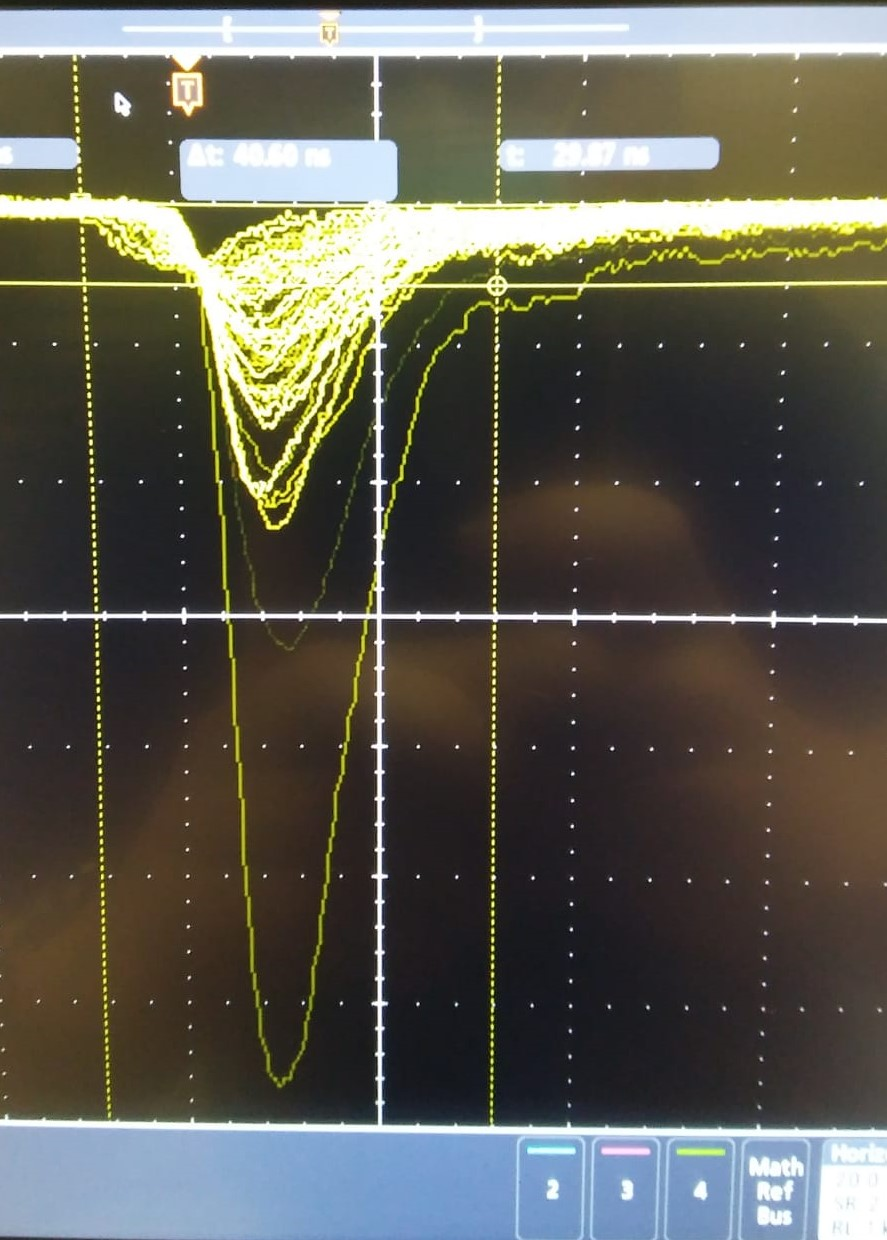
\includegraphics[scale=0.2]{./immagini/TimeOfFlight/SegnaliOsc.jpg}
\caption{Divisioni: $\frac{10ns}{div}$ nei tempi $\frac{20mV}{div}$ per i voltaggi}
\label{fig:SegnaliOsc}
\end{center}
\end{figure}

La scelta del tempo di lunghezza del segnale output del discriminatore è stata fatta osservando la durata dei tempi di un singolo impulso ($\sim 15$ massimo $20 ns$ come da figura \ref{fig:SegnaliOsc}) al quale però è stato pensato di aggiungere un possibile ritardo dovuto alla differenza di trasmissione. Inoltre dovendo misurare dei ritardi di qualche ns tra due o più segnali, quindi non in coincidenza quasi istantanea sono stati stimati i possibili tempi di percorrenza delle particelle

\begin{itemize}
\item Il primo ritardo è dovuto alla velocità della luce nella barra scintillante lunga: v$_{teorica} = \frac{30\frac{cm}{ns}}{n} = 19 \frac{cm}{ns}$, perciò si ha un ritardo massimo di $\frac{L = 280 [cm]}{v = 19 [\frac{cm}{ns}]} \simeq 15 ns$
\item il secondo ritardo è quello dovuto al tempo di volo delle particelle. La distanza massima che percorrono le particelle è di circa: $d = \sqrt{\frac{L}{2}^2 + h^2} \simeq 224 cm$, e supponendo una velocità di $10\frac{cm}{ns}$ si ottiene un ritardo di $\sim 21 ns$
\end{itemize}

Dopo aver visualizzato i segnali di figura \ref{fig:SegnaliOsc} sono stati scelti i seguenti livelli di discriminazione:

\begin{itemize}
\item -45mv in ampiezza
\item 50 ns in larghezza di tempi
\end{itemize}

\subsection{Alimentazione}
\label{sec:CalSin}
Sono state ricercate le alimentazioni dei PMT-3 e PMT-1

\begin{figure}[H]
	\centering
	\begin{subfigure}[b]{0.4\textwidth}
		\centering
		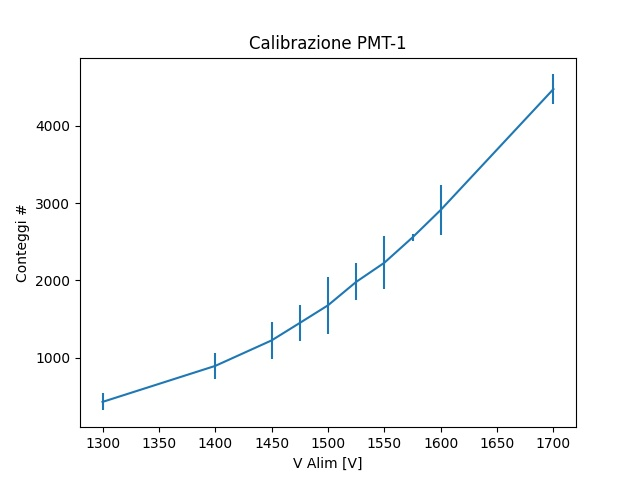
\includegraphics[width=\textwidth]{./immagini/TimeOfFlight/CalSinPMT-1.jpg}
		\caption{Gli errori in figura sono moltiplicati per 10}
		\label{fig:CalSinPMT-1}
	\end{subfigure}
	\hfill
	\begin{subfigure}[b]{0.4\textwidth}
		\centering
		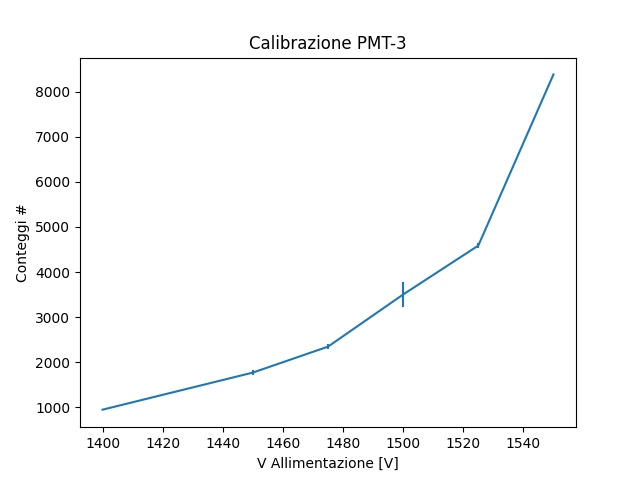
\includegraphics[width=\textwidth]{./immagini/TimeOfFlight/CalSinPMT-3}
		\caption{}
		\label{fig:CalSinPMT-3}
	\end{subfigure}
	\caption{Calibrazioni dei PMT presi individualmente. I conteggi sono stati presi per 10 secondi}
	\label{fig:CalSinPMT}
\end{figure}

Non avendo osservato un evidente plateau in nessuno dei due grafici (vedi figura \ref{fig:CalSinPMT}) è stato scelto di alimentarli inizialmente tutti con una tensione di 1600V

\subsection{Coincidenze}
\label{sec:Coinc}
Per la massimizzazione delle coincidenze sono state fatte due prova la prima ricercando un Plateau nel rapporto tra coincidenze, la seconda invece andando a massimizzare l'efficienza osservando che i conteggi in singola non aumentassero di troppi ordini di grandezza

\begin{figure}
\centering
\title{Coincidenze su oscilloscopio}
\begin{center}
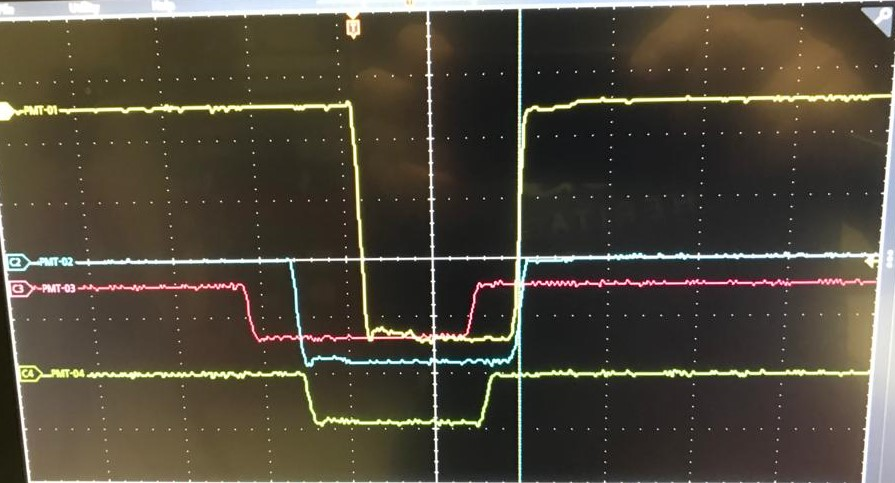
\includegraphics[scale=0.35]{./immagini/TimeOfFlight/CoincOscill.jpg}
\caption{In giallo il segnale della coincidenza tripla. Verde e blu PMT collegati alla barra scintillante Rosso PMT-3. Trigger impostato sulla coincidenza tripla}
\label{fig:ExCoinc}
\end{center}
\end{figure}

\subsubsection{Ricerca Plateau}
Per primo è stato calibrato il PMT-1 dove:\\
Le coincidenze doppie sono C$_{23}$\footnote{Con C$_{ijk}$ si indica una coincidenza tra i segnali raccolti dai PMT numerti con i, j e k} e le triple C$_{123}$\\
$V_{Alim2}=V_{Alim3}=1600V$\\
Soglie impostate a $\sim-45mV$ per i PMT-1e2 e $\sim-50mV$ per il PMT-3

\begin{figure}[H]
\centering
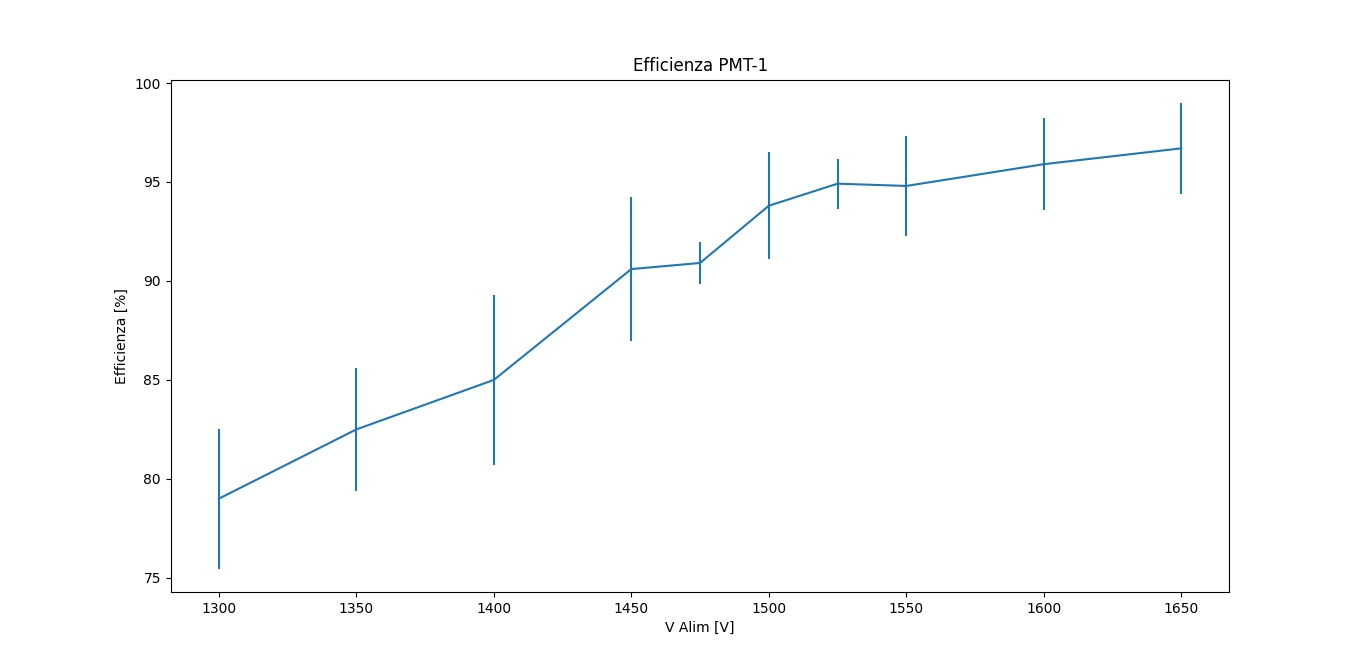
\includegraphics[scale=0.3]{./immagini/TimeOfFlight/EffPMT145mV}
\caption{Per gli errori è stato considerato l'errore di efficienza dovuto ad una distribuzione binomiale: $\sigma = \sqrt{\frac{\epsilon(1-\epsilon)}{N}}$, dove $\epsilon = \frac{n}{N}$, n è il numero di occorrenze positive e N quello totale}
\label{fig:EffPMT145mV}
\end{figure}

Osservando la figura \ref{fig:EffPMT145mV} è stata selezionata un'alimentazione di 1510 per un'efficienza del 93.8$\%$ per il PMT-1.\\
Questa scelta però può essere limitante, facendo un stima delle coincidenze casuali si nota infatti che, anche con un'efficienza ritenuta alta del 96$\%$ sono comunque molto basse:

\begin{equation}
f_{cas} = f_1 f_2 f_3 \tau _1\tau _2 \simeq (5*10^2)(5*10^2) 10^3 (50*10^{-9})^2 = 6,25*10^{-7} cps
\label{eq:CoinCasPMT1Prova1}
\end{equation}

\subsubsection{Massimizzazione dell'efficienza}
Per questo metodo di calibrazione è stato tenuto il PMT-3 nel centro della barra scintillante e alla stessa altezza e a turno è stato calcolato il rapporto tra coincidenze doppie e triple per PMT-1 e 2.\\
Si sceglie una tensione di alimentazione che corrisponda ad un'efficienza del 98$\%$.

\paragraph{PMT-2; Scelta soglia discriminazione}
Per la prima calibrazione (PMT-2) si è verificata una possibile dipendenza della curva di efficienza dal valore di soglia impostato con il modulo NIM discriminatore.

\begin{figure}[H]
     \begin{subfigure}[b]{0.49\textwidth}
         \centering
         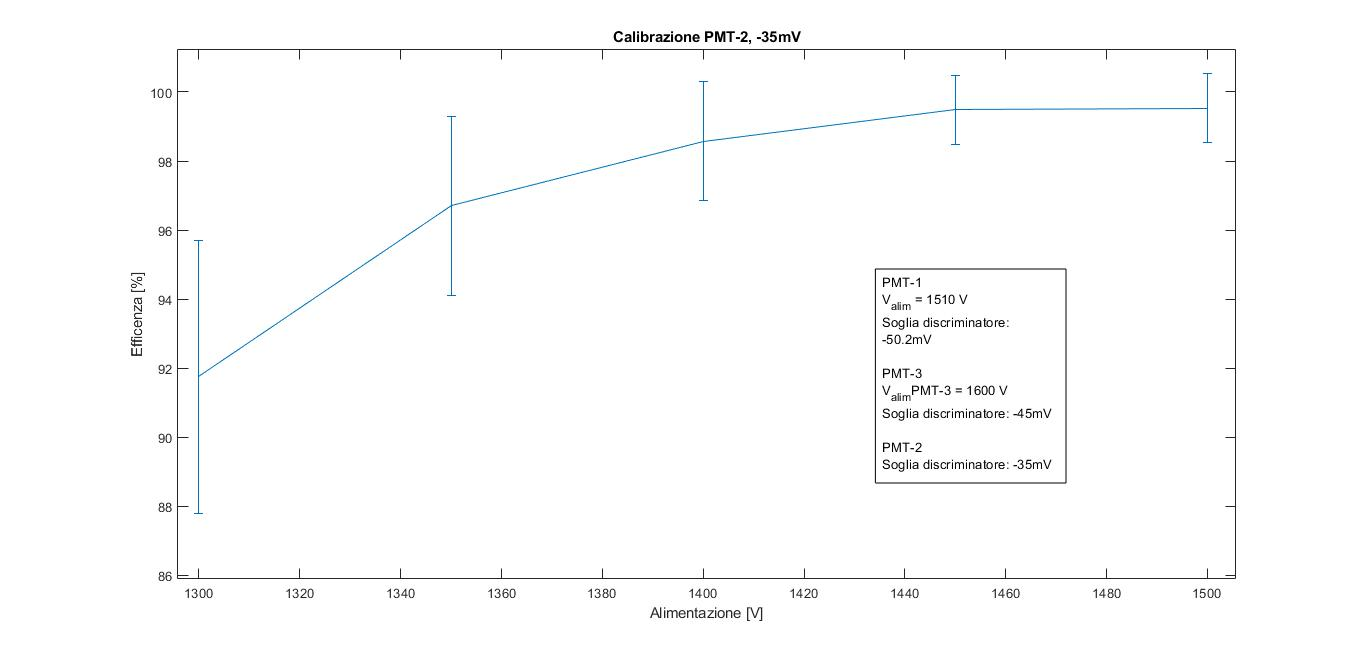
\includegraphics[width=\textwidth]{./immagini/TimeOfFlight/EffPMT235mV.jpg}
         \caption{}
         \label{fig:EffPMT235mV}
     \end{subfigure}
     \hfill
     \begin{subfigure}[b]{0.49\textwidth}
         \centering
         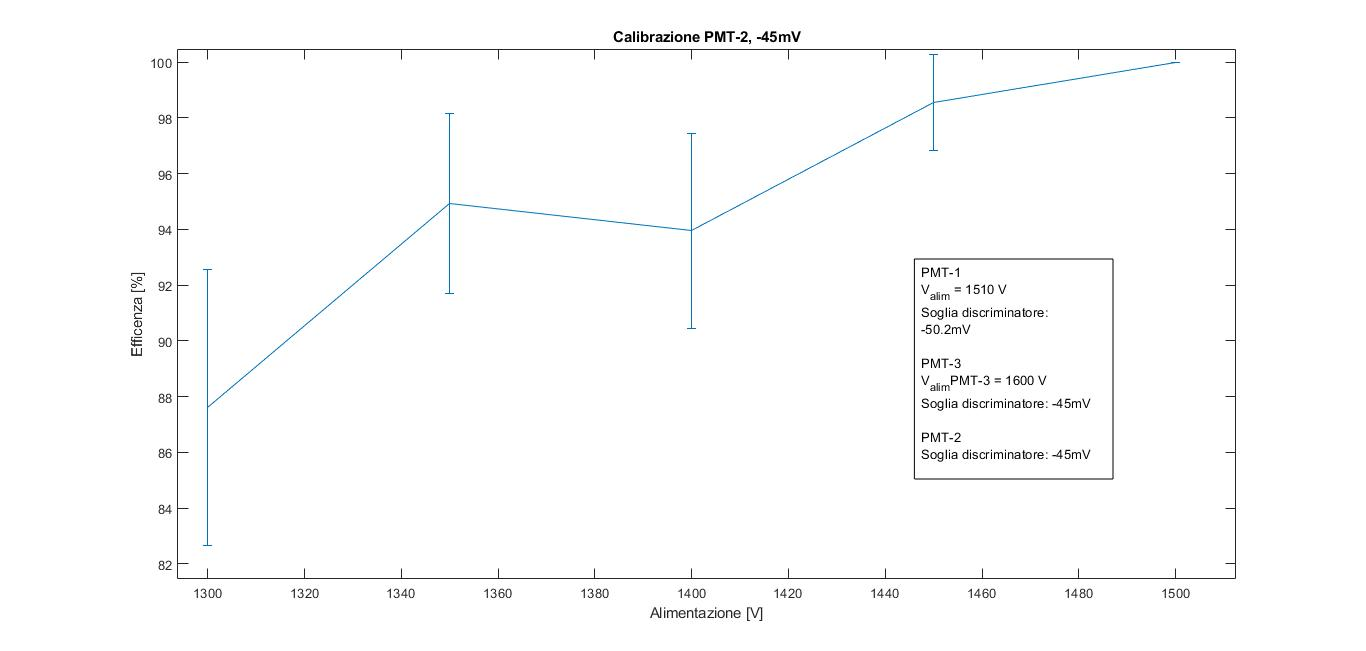
\includegraphics[width=\textwidth]{./immagini/TimeOfFlight/EffPMT245mV.jpg}
         \caption{}
         \label{fig:EffPMT245mV}
     \end{subfigure}
     \caption{Efficienze del PMT-2 con due livelli di soglia differente: -35mV \ref{fig:EffPMT235mV}, -45mV \ref{fig:EffPMT245mV}}        
     \label{fig:EffPMT2SoglieDis}
\end{figure}

Nei due tentativi a soglie diverse si nota che quando si raggiunge l'efficienza desiderata del 98$\%$ si hanno i seguenti conteggi in singola:

\begin{tabular}{|c|c|c|c|c|}
\hline
Soglia [mV] & V$_{Alim}$ [V] & cps PMT-1 & cps PMT-2 & cps PMT-3\\
\hline
-35 & 1400 & 149 & 142 & 986\\
\hline
-45 & 1450 & 150 & 142 & 852\\
\hline
\end{tabular}

Non essendoci differenze sostanziali abbiamo preferito la scelta con: soglia = -35mV; V$_{Alim_2}$ = 1400V

\paragraph{PMT-1, soglia -35mV}
Per il PMT-1 è stata tenuta solamente la soglia a -35 così da tenerlo simile al PMT-2

\begin{figure}[H]
\centering
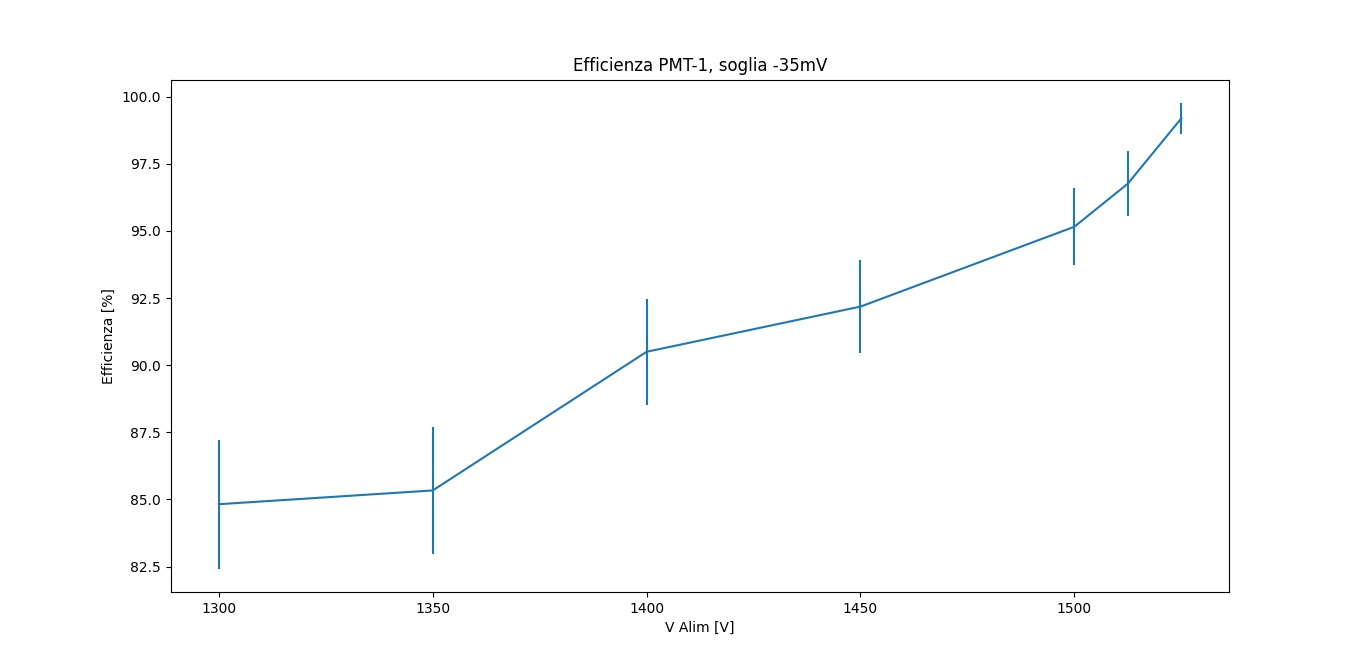
\includegraphics[scale=0.3]{./immagini/TimeOfFlight/EffPMT135mV}
\caption{Per un valore di alimentazione di 1550V sono state trovate un numero maggiore di triple rispetto alle doppie}
\label{fig:EffPMT135mV}
\end{figure}

Facendo riferimento alla figura \ref{fig:EffPMT135mV} è stato deciso di alimentare il PMT-1 con V$_{Alim_1}$ = 1525V


\paragraph{PMT-4}
\label{sec:CalPMT-4}
Per questa calibrazione abbiamo posizionato lo scintillatore 3 esattamente sopra lo scintillatore 4 come in figura \ref{fig:PMT3posPMT4}.\\
Le doppie tra segnali del PMT-3 e PMT-2, le triple con il PMT-4

\begin{figure}[H]
\centering
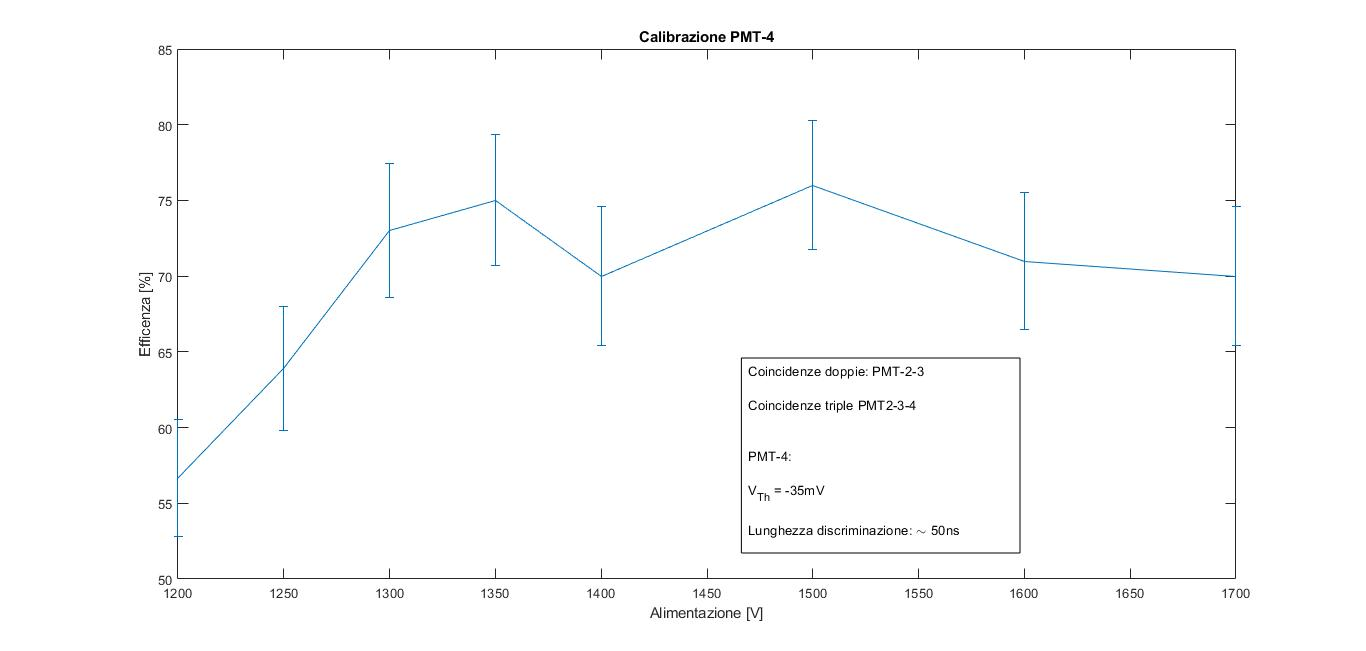
\includegraphics[scale=0.25]{./immagini/TimeOfFlight/CoincidenzePMT4.jpg}
\caption{I segnali del PMT-4 sono stati discriminati con una soglia a -35mV e una lunghezza di discriminazione di 50ns}
\label{fig:EffPMT4}
\end{figure}

Notiamo che nonostante lo scintillatore 4 sia notevolmente più grande del 3 l'efficienza è ben diversa da quella attesa del 100$\%$ ma si stabilizza all'incirca sul 70$\%$.

\begin{figure}[H]
\centering
\title{Posizione PMT-3 e PMT-4}
\begin{center}
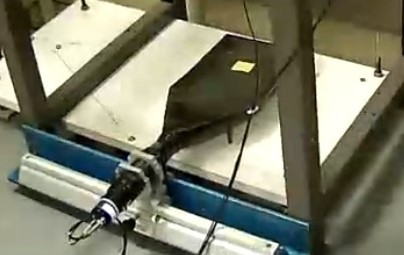
\includegraphics[scale=0.4]{./immagini/TimeOfFlight/CalPMT4app.jpg}
\caption{Il PMT-4 è posto sotto del legno, ne è purtroppo poco visibile il perimetro segnato a matita}
\label{fig:PMT3posPMT4}
\end{center}
\end{figure}

I problemi potrebbero essere dovuti a parti elettroniche, connessioni o ad effetti fisici, non sicuramente geometrici.\\
La scelta è stata presa scegliendo un valore di alimentazione che si avvicinasse ai fotomoltiplicatori precedenti e che fosse comunque relativamente massima con conteggi dell'ordine del centinaio di Hz:

\begin{tabular}{|c|c|c|c|c|c|c|c|}
\hline
V$_{Alim} [V]$ & doppie & triple & Cont. PMT-1 & Cont. PMT-2 & Cont. PMT-3 & Cont. PMT-4 & Tempo [ms]\\
\hline
1400 & 100 & 84 & 668883 & 48185 & 135507 & 92826 & 273037\\
\hline
1350 & 100 & 67 & 62857 & 41377 & 168528 & 86412 & 349377\\
\hline
\end{tabular}

in entrambi i casi si rimane su valori delle centinaia di cps. Si sceglie di alimentare con 1400V  ($\sim$340cps)

\section{Velocità della luce nella barra scintillante}
\label{sec:VLuce}
\subsection{Cenni teorici}
Ogni volta che una particella carica attraversa la barra scintillante questa rilascia energia eccitando gli elettroni degli atomi reticolari; successivamente per diseccitamento vengono liberati fotoni che formeranno un fascio luminoso. Questo segnale luminoso deve attraversare la lunghezza dello scintillatore plastico per raggiungere uno dei due capi e poter essere rivelato dal fotomoltiplicatore.\\
La luce essendo in un mezzo fisico e non nel vuoto andrà ad una velocità ridotta del valore dell'indice di rifrazione del materiale n$\simeq$ 1.58. Quindi v$_{luce} = \frac{30}{1,58} \simeq 19,0 \frac{cm}{ns}$

\subsection{Misure}
Per la velocità dei segnali all'interno della barra scintillante lunga abbiamo posizionato il PMT-3 in diversi punti della barra così da fissare la distanza percorsa dalla luce e abbiamo associato la velocità seguendo questa formula.\\
I ritardi tra i segnali letti dai PMT sono stati presi direttamente tramite oscilloscopio
\begin{equation}
\Delta t = \frac{2x-L}{v} + (\tau_1 - \tau_2)
\label{eq:VLuceBarra}
\end{equation}
dove L è la lunghezza della barra (280 cm) $\Delta t$ il ritardo tra i segnali che leggiamo da oscilloscopio, x la posizione che scegliamo in base a dove poniamo il PMT-3, $\tau_1$ e $\tau_2$ dei possibili ritardi tra le trasmissioni dei segnali che vanno ad influire unicamente sull'offset della retta.\\
L'inverso del coefficiente angolare sarà la nostra velocità.\\
L'errore associato alla posizione del PMT-3 è dato dalla larghezza dello scintillatore 3 (22cm) divisa $\sqrt{12}$($\sigma _x = \frac{22}{\sqrt{12}}$) poiché assumiamo che la probabilità che una particella attraversi il materiale è uniforme su tutta la larghezza del rivelatore.


\subsection{Analisi dati, Oscilloscopio}
Sono stati presi 100 di questi eventi tripli per ognuna delle posizioni scelte e ne è stata presa direttamente media e devstd prodotta dall' oscilloscopio. A quel punto ne è stato fatto un fit con la retta in equazione \ref{eq:VLuceBarra}

\begin{figure}[H]
     \centering
     \begin{subfigure}[b]{0.47\textwidth}
         \centering
         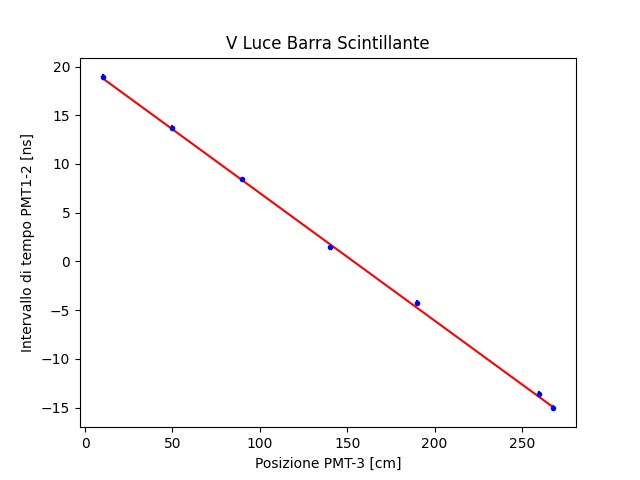
\includegraphics[width=\textwidth]{./immagini/TimeOfFlight/VLightBarra.jpg}
         \caption{I dati sono stati fittati utilizzando l'equazione \ref{eq:VLuceBarra}}
         \label{fig:FitVLightBarra}
     \end{subfigure}
     \hfill
     \begin{subfigure}[b]{0.47\textwidth}
         \centering
         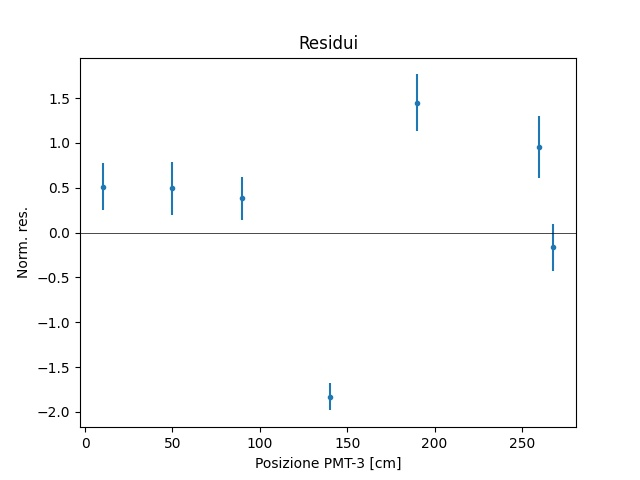
\includegraphics[width=\textwidth]{./immagini/TimeOfFlight/ResVLightBarra.jpg}
         \caption{}
         \label{fig:ResVLIghtBarra}
     \end{subfigure}
     \caption{Negli errori è stata considerata anche l'incertezza sulla posizione dovuta alla larghezza dello scintillatore 3: $\sigma = \sqrt{(\sigma _y)^2 + (\frac{\delta f(x_i)}{\delta x}\sigma _x)^2}$}        
     \label{fig:FitLinVLightBarra}
\end{figure}

Dal fit abbiamo ottenuto i seguenti risultati\footnote{Chi2 = 7,04, ndof= 5, norm cov= 0.86}:

\begin{tabular}{|c|c|}
\hline
v [$\frac{cm}{ns}$] & off [ns] \\
\hline
-15,28 $\pm$ 0,16 & 20,10 $\pm$ 0,22\\
\hline
\end{tabular}

Il segno meno è dovuto alla scelta della differenza tra i PMT-1 e PMT-2.

\subsection{Analisi dati ADC}
Per questa analisi abbiamo preso diversi segnali in coincidenza tra PMT 1-2 e 3 posizionato in alcune posizioni della barra e fatto media e devstd dei $\Delta t$ ricavati

\begin{figure}[H]
     \begin{subfigure}[b]{0.47\textwidth}
         \centering
         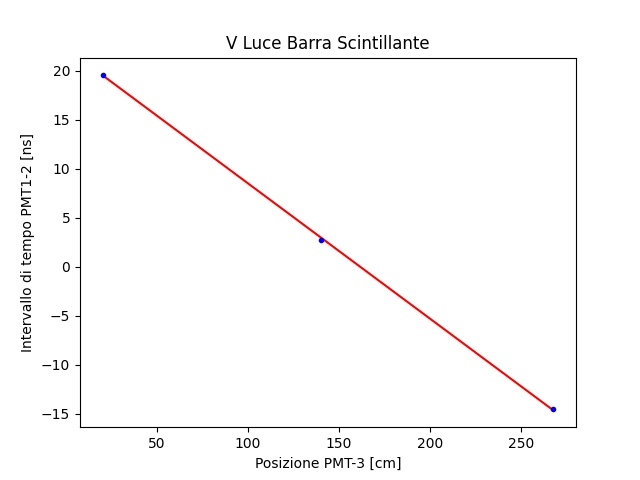
\includegraphics[width=\textwidth]{./immagini/TimeOfFlight/VLightBarraADC}
         \caption{}
         \label{fig:FitVLightBarraADC}
     \end{subfigure}
     \hfill
     \begin{subfigure}[b]{0.47\textwidth}
         \centering
         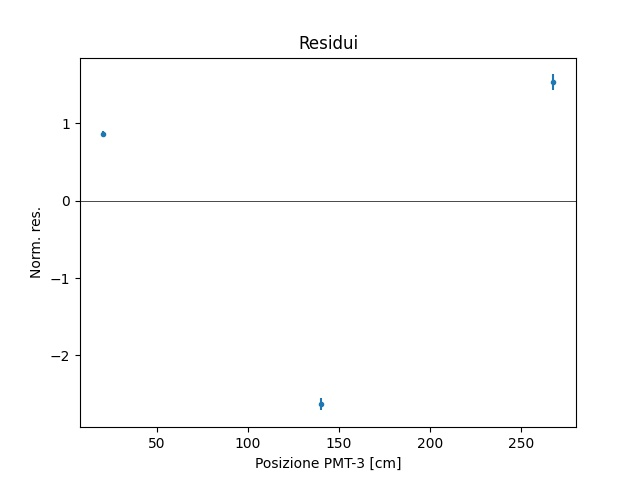
\includegraphics[width=\textwidth]{./immagini/TimeOfFlight/ResVLightBarraADC}
         \caption{Negli errori è stata considerata anche l'incertezza sulla posizione dovuta alla larghezza dello scintillatore 3: $\sigma = \sqrt{(\sigma _y)^2 + (\frac{\delta f(x_i)}{\delta x}\sigma _x)^2}$}
         \label{fig:ResVLIghtBarraADC}
     \end{subfigure}
     \caption{}        
     \label{fig:FitLinVLightBarraADC}
\end{figure}

Dal fit abbiamo ottenuto i seguenti risultati\footnote{Chi2 = 10,01, ndof = 1, norm cov= 0.64}:

\begin{tabular}{|c|c|}
\hline
v [$\frac{cm}{ns}$] & off [ns] \\
\hline
-14,50 $\pm$ 0,16 & 22,31 $\pm$ 0,19\\
\hline
\end{tabular}

\section{Misura della distribuzione di V}
\label{sec:MisuraVMu}
\subsection{Cenni Teorici}
L'obiettivo di questa sezione è quello di misurare la distribuzione di velocità delle particelle cosmiche che riveliamo grazie all'apparato descritto in sezione \ref{sec:AppSper}.\\
I muoni hanno vita media molto breve e se visti dal sistema di riferimento nel quale la particella si trova a riposo anche se si muovessero alla velocità della luce questi non raggiungerebbero la Terra. Invece se visti da un osservatore esterno questi per la dilatazione temporale raggiungono il livello del mare.\\
Dopo aver ricostruito la distribuzione di velocità di questi eventi saranno posizionate delle lastre di Piombo sulla traiettoria delle particelle, i Muoni essendo particelle cariche (carica -e) quando attraversano un mezzo perdono una quantità di energia per unità di lunghezza che segue la curva descritta dall'espressione nota come la "Bethe-Block". Secondo questa curva le particelle con poca energia perdono una quantità di energia maggiore rispetto a quelle più veloci\footnote{Qua mi riferisco unicamente alla parte di curva prima del minimo che si trova intorno a circa 3-4$\beta \gamma$}.\\
Quindi si ricostruirà un secondo grafico di distribuzione delle velocità delle particelle che avranno attraversato il piombo e sarà confrontato con il primo.
\subsection{Set-up}
Per questo intento si tiene il PMT-3 centrato sopra lo scintillatore 4 come in figura \ref{fig:PMT3posPMT4}\\
Il tempo di volo e dunque la velocità sarà misurata rispetto al PMT-3 in quanto potrebbe avere una risposta più veloce rispetto al più grande PMT-4 che inoltre ha presentato un difetto in efficienza non di poco conto (vedi \ref{sec:CalPMT-4}). La distanza tra PMT-4 e PMT-3 è molto piccola rispetto ad h e non influirebbe su una misura di TOF fatta con i segali del PMT-4.\\
Il piombo sarà posizionato tra PMT3 e 4.\\
Per queste prese dati ci serviremo dell'ADC converter.
\paragraph{ADC Converter}
Alcune caratteristiche che hanno Influenzato notevolmente la fase di analisi dati\footnote{vedi l'appendice \ref{secA:ProblemiADC}}
\begin{itemize}
\item Frequenza campionamento 250MHz, un campione ogni 4 ns
\item Lunghezza singolo record 1030 dati, 4120 ns
\end{itemize}

\subsection{Calcoli}
\label{sec:CalcoliVMu}
Considerando il tempo t$_0$ come quello in cui una particella attraversa istantaneamente la barra scintillante\footnote{Se consideriamo anche una velocità di 10$\frac{cm}{ns}$, che a posteriori è molto bassa, in realtà passa dal centro della barra dopo una frazione di ns}, scriviamo i tempi t$_i$, ovvero i tempi necessari ai vari PMT-i di ricevere i segnali e inviarli agli apparecchi di presa dati.\\
Consideriamo inoltre il centro della barra il punto $x = 0$.\footnote{Sulla barra scintillante dell'esperienza il centro corrispondeva a 140cm di distanza dal PMT-1}
\begin{equation}
t_1 = t_0 + \frac{x}{v_l} + \tau_1
\end{equation}
\begin{equation}
t_2 = t_0 - \frac{x}{v_l} + \tau_2
\end{equation}
\begin{equation}
t_3 = t_0 + TOF + \tau_3
\label{eq:TempiPMT}
\end{equation}

dove $\tau_i$ sono i vari ritardi dovuti esclusivamente alla trasmissione indica il tempo necessario al segnale luminoso di andare dal punto di incidenza al fotocatodo del PMT, si assume il PMT-3 Prompt, $v_l$ la velocità della luce nella barra scintillante misurata nella sezione \ref{sec:VLuce} e TOF il tempo di volo di una particella.\\
Da questi 3 tempi troviamo un'espressione che leghi prima i $\Delta t$ misurabili alla posizione di passaggio della particella nella barra e successivamente alla velocità delle particelle\footnote{Nelle seguenti espressioni appariranno termini come $\Delta t_{31}$ o come R$_{12}$, in questi casi si deve fare attenzione all'ordine delle cifre. Per esempio R$_{12}$= $\tau_1$ - $\tau_2 \neq \tau_2 - \tau_1$ = R$_{21}$ quindi $R_{12}=-R_{21}$}

\begin{equation}
\Delta t_{12} = t_1 - t_2 = t_0 + \frac{x}{v_l} + \tau_1 - t_0 + \frac{x}{v_l} - \tau_2 = 2\frac{x}{vl} + R_{12}
\end{equation}
\begin{equation}
\Delta t_{31} = t_3 - t_1 = t_0 + TOF + \tau_3 - t_0 - \frac{x}{v_l} - \tau_1 = TOF - \frac{x}{v_l} R_{31}
\end{equation}
\begin{equation}
\Delta t_{32} = t_3 - t_2 = t_0 + TOF + \tau_3 - t_0 + \frac{x}{v_l} - \tau_2 = TOF + \frac{x}{v_l} R_{32}
\end{equation}

Quindi per la posizione abbiamo:

\begin{equation}
x = (\Delta t_{12} - R_{12})\frac{v_l}{2}
\label{eq:PosX}
\end{equation}

Per i tempi di volo possiamo utilizzare sia il ritardo $\Delta t_{31}$ che $\Delta t_{32}$ oppure mediare i tempi di volo per ricavare un'espressione indipendente dal calcolo della posizione ma unicamente dalle misure sui $\Delta t$:

\begin{equation}
TOF_1 = \Delta t_{31} + \frac{x}{v_l} - R_{31}
\label{eq:TOF1}
\end{equation}
\begin{equation}
TOF_2 = \Delta t_{32} + \frac{x}{v_l} - R_{32}
\label{eq:TOF2}
\end{equation}
\begin{equation}
TOF = \frac{TOF_1 + TOF_2}{2} = \frac{\Delta t_{31} + \Delta t_{32} - R_{31} - R_{32}}{2}
\label{eq:TOF}
\end{equation}

La velocità sarà dato da:

\begin{equation}
v = \frac{d}{TOF} = \frac{\sqrt{x^2+h^2}}{TOF}
\label{eq:VMu}
\end{equation}

dove h è l'altezza della barra scintillante dal PMT-3, x la posizione rispetto al centro della barra scintillante e possiamo scegliere una delle misure di tempo di volo in equazioni \ref{eq:TOF1},\ref{eq:TOF2},\ref{eq:TOF}

\subsection{Misure}
\label{sec:MisureV}
\paragraph{Misura del TimeStamp}
Per misurare l'istante in cui passa un segnale (50$\%$ del minimo del segnale) è stato considerato il baricentro della discesa del segnale con qualche dato in più sia a tempi maggiori del minimo che a tempi minori dell'inizio del segnale. In particolare un campione prima della partenza del segnale e 3 dopo il minimo del segnale\footnote{Vedi appendice \ref{secA:Scelta}}

\paragraph{Ritardi R$_{ij}$; i,j=1,2,3}
Per misurare i Ritardi dovuti alla trasmissione del segnale (R$_{ij}$ in equazione \ref{eq:VMu}) è stato posizionato il PMT-3 sul centro della barra scintillante lunga triggerando sulle triple C$_{123}$

\begin{figure}[H]
\centering
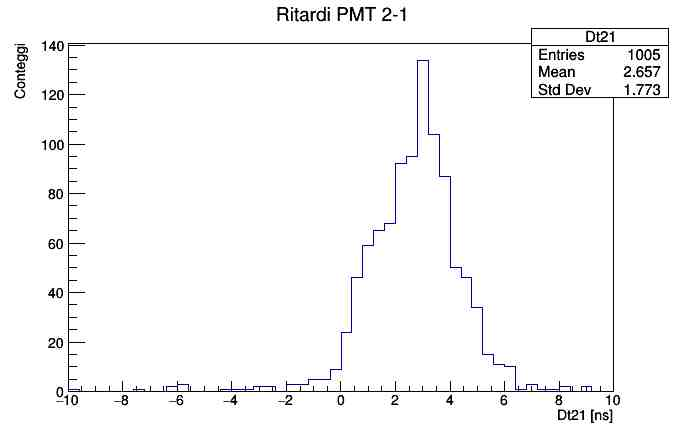
\includegraphics[scale=0.3]{./immagini/TimeOfFlight/Rit21Fore.jpg}
\caption{}
\label{fig:Dt21Fore}
\end{figure}

Per ogni istogramma come quello di figura \ref{fig:Dt21Fore} sono stati eseguiti dei fit con una gaussiana per stimare i ritardi tra i PMT

\begin{tabular}{|c|c|c|}
\hline
Rit 2-1 [ns] & Rit 3-1 [ns] & Rit 3-2 [ns] \\
\hline
2,74 $\pm$ 1,42 & -10,0 $\pm$ 1,48 & -12,8 $\pm$ 1.65\\
\hline
\label{tab:RitFore}
\end{tabular}

E dunque la distribuzione di velocità è

\begin{figure}[H]
\centering
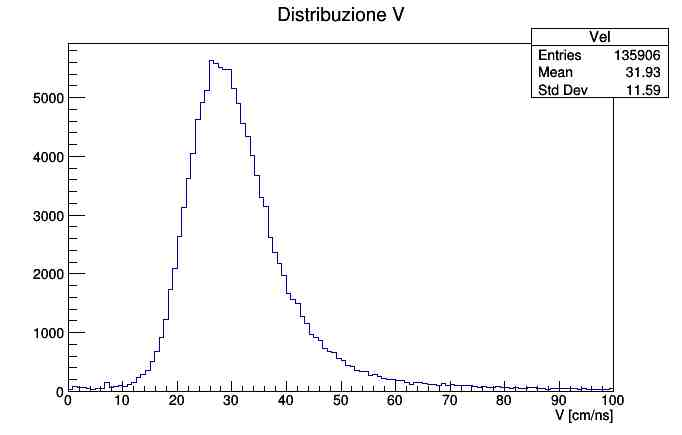
\includegraphics[scale=0.4]{./immagini/TimeOfFlight/VTripleFore.jpg}
\caption{In questo istogramma sono stati usati tutti i dati a nostra disposizione anche di prese dati differenti}
\label{fig:VFore}
\end{figure}

\subsection{Eventi Ultrarelativistici e non}
\label{sec:RapportoU-N}
\paragraph{Conti sul Piombo}
Osservando la figura \ref{fig:VFore} è stato deciso di tagliare gli eventi con velocità inferiore a 20$\frac{cm}{ns}$
\begin{center}
$v = 20\frac{cm}{ns} \Rightarrow \beta \simeq \frac{2}{3} \Rightarrow \gamma \simeq 1,3$ \\ $ p=\gamma m \beta \simeq 94.5 \frac{MeV}{c} $
\end{center}

Dal sito PDG\footnote{In particolare alla pagina \url{https:pdg.lbl.gov/2020/AtomicNuclearProperties/MUE/muE_lead_Pb.pdf}, pagina relativa a come si comportano i muoni in funzione della loro energia nel piombo} si vede che impulsi di circa 100MeV per essere teoricamente frenati necessitano di uno spessore di Piombo (per unità di densità, CSDA range) di 1,521 $\frac{g}{cm^2}$, perciò sapendo che la densità del piombo vale 11,35 $\frac{g}{cm^3}$ si ricava che per frenare le particelle con $v<20\frac{cm}{ns}$ servono almeno 1,2-1,4 cm di piombo.\\
Così sono state posizionate tra il PMT-3 e PMT-4 7 lastre di piombo di 2 cm ciascuna

\paragraph{2 Metodi}
Data la bassa efficienza del PMT-4 sono stati pensati due metodi per valutare la quantità di particelle che vengono assorbite dalle lastre di Piombo.\\
Il primo metodo è quello di confrontare due istogrammi normalizzati di quadruple senza piombo e quadruple con il piombo\footnote{Per quadruple intendiamo coincidenze tra tutti i 4 PMT, C$_{1234}$}. In questa maniera si eviterebbe il problema di conteggi minori dovuti all'efficienza del PMT-4.\\
In alternativa si potrebbe stimare l'efficienza del PMT-4 tramite coincidenze triple e quadruple di una presa dati senza piombo lungo la traiettoria, e successivamente si misureranno i rapporti tra coincidenze Triple e Quadruple con il Piombo dividendo per l'efficienza precedentemente stimata.

\subsubsection*{Metodo 1, Rapporto quadruple normalizzate}

\begin{figure}[H]
\centering
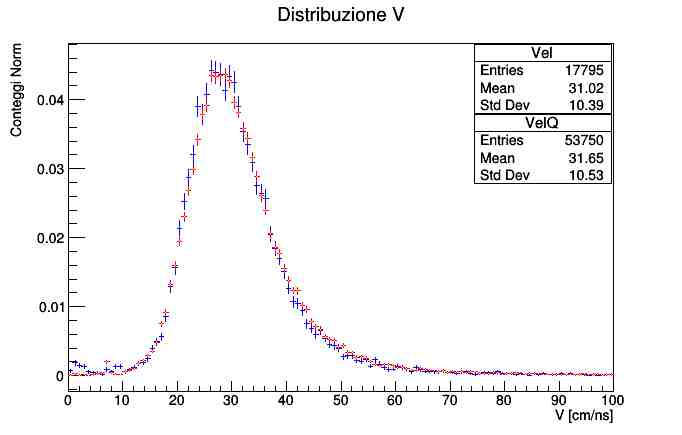
\includegraphics[scale=0.3]{./immagini/TimeOfFlight/VNormForeQuadruple.jpg}
\caption{In blu la distribuzione normalizzata delle velocità degli eventi senza piombo, in rosso con il piombo. Integrale sotto il grafico $\sim$0,97 per entrambe le distribuzioni}
\label{fig:VNormFore}
\end{figure}

\'E stato eseguito un fit dei dati di V di figura \ref{fig:VNormFore}, considerando i dati più vicini ad assomigliare ad una gaussiana\footnote{é stato scelto il range nelle ascisse in base alla DevStd segnata in figura. \'E stato scelto di fare un fit della curva compresa entro 2 sigma dalla media, perciò circa compresa tra 5 e 55 $\frac{cm}{ns}$}. Media e deviazione standard sono riportate in tab \ref{tab:FitVMet1}

\begin{tabular}{c|c}
C$_{1234}$ senza Pb [$\frac{cm}{ns}$] & 29,6 $\pm$ 6,9 \\
\hline
C$_{1234}$ con Pb[$\frac{cm}{ns}$] & 30,1 $\pm$ 7,3
\label{tab:FitVMet1}
\end{tabular}

\begin{figure}[H]
\centering
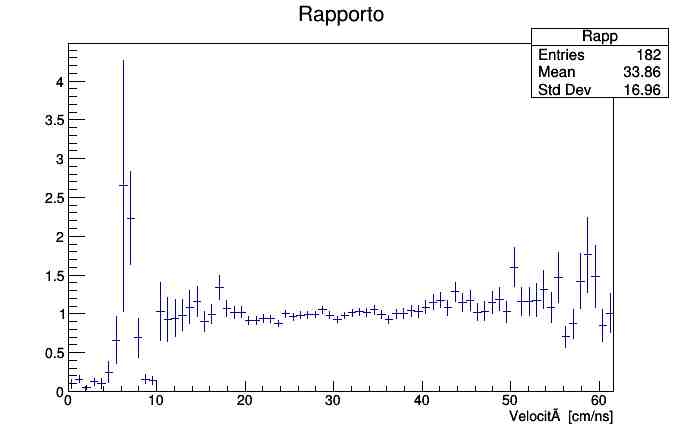
\includegraphics[scale=0.3]{./immagini/TimeOfFlight/VRappFore.jpg}
\caption{Rapporto $\frac{quadruple con Pb}{Quadruple senza Pb}$.}
\label{fig:VRappFore}
\end{figure}

\subsubsection*{Metodo 2, Misura dell'efficienza}
\label{sec:Met2}
Si prova questo metodo per poter utilizzare lo stesso set di eventi così da evitare problemi di incontrare statistiche molto lontane tra loro

\paragraph{Efficienza PMT-4}
Sapendo che le quadruple lette valgono:
\begin{equation}
N_{Quadruple} = N_{Triple} * N_{Eventi positivi} * Eff
\end{equation}
Allora il numero di eventi che passano il Pb vale:
\begin{equation}
N_{Eventi positivi} = \frac{N_{Quadruple}}{N_{Triple}*Eff}
\label{eq:VRappMet2}
\end{equation}

\begin{figure}[H]
\centering
\begin{subfigure}[b]{0.4\textwidth}
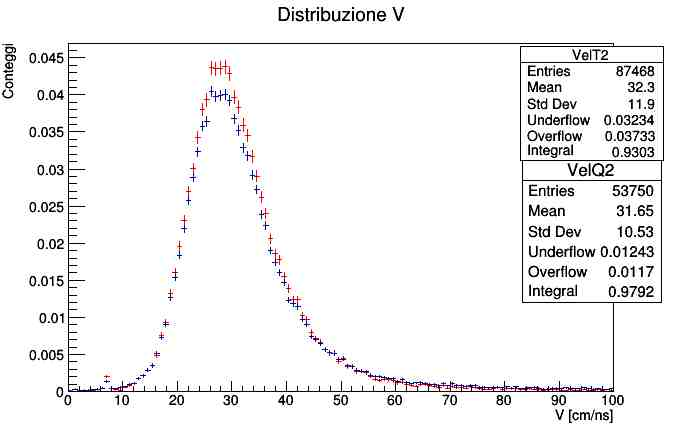
\includegraphics[width=\textwidth]{./immagini/TimeOfFlight/VNormQuad2.jpg}
\caption{In rosso i dati delle quadruple, in blu le triple}
\label{fig:DistrVPb2Fore}
\end{subfigure}
\hfill
\begin{subfigure}[b]{0.4\textwidth}
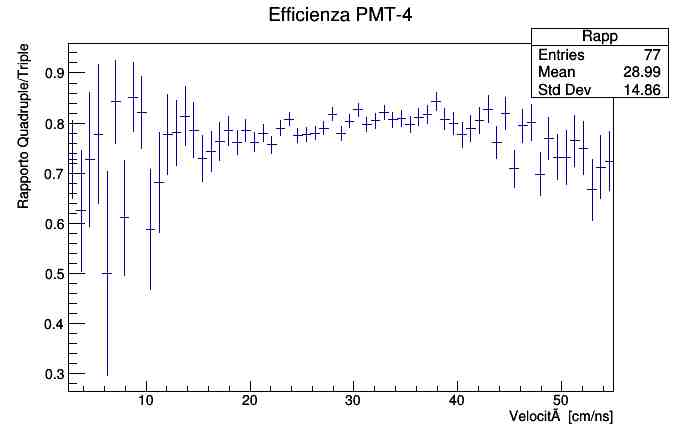
\includegraphics[width=\textwidth]{./immagini/TimeOfFlight/EffFore.jpg}
\caption{Rapporto $\frac{Quadruple}{Triple}$ senza Piombo tra i PMT. Gli errori sono stati valutati con la formula: $\sigma _{eff} = \sqrt{eff(1-eff)/N_{Triple}}$}
\label{fig:EffFore}
\end{subfigure}
\end{figure}

Dalla figura \ref{fig:EffFore} si misura un'efficienza per il PMT-4 di circa il 79$\%$, stimata tramite fit di una retta costante su tutti i dati.\\
Da due fit sui dati in figura \ref{fig:DistrVPb2Fore} delle triple e delle quadruple si nota che le velocità medie sono tra loro confrontabili; 30,0$\pm$ 7,2 $\frac{cm}{ns}$ per entrambe le curve.\\
Infine eseguendo il rapporto tra gli istogrammi e dividendolo per l'efficienza(come da equazioni \ref{eq:VRappMet2}) otteniamo i seguenti grafici(\ref{fig:RappPbFore} e \ref{fig:RappPbEffFore}):

\begin{figure}[H]
\begin{subfigure}[b]{0.4\textwidth}
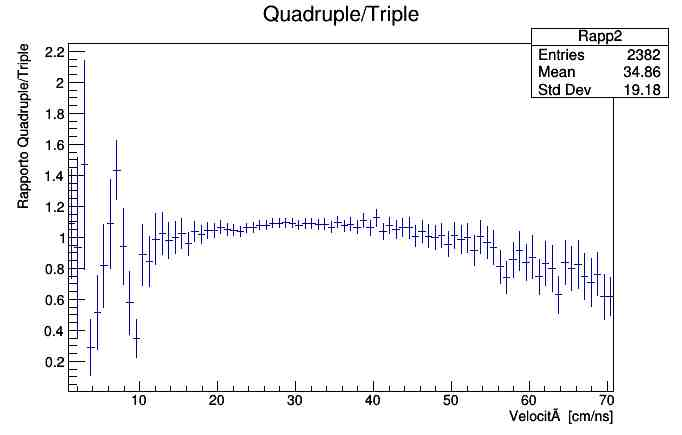
\includegraphics[width=\textwidth]{./immagini/TimeOfFlight/RappPiomboFore.jpg}
\caption{}
\label{fig:RappPbFore}
\end{subfigure}
\hfill
\begin{subfigure}[b]{0.4\textwidth}
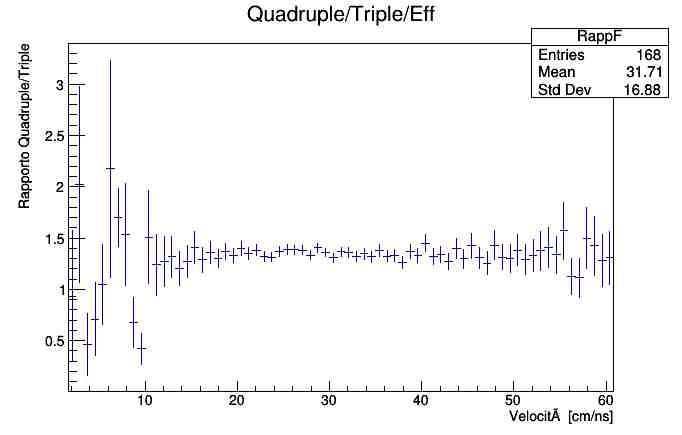
\includegraphics[width=\textwidth]{./immagini/TimeOfFlight/RappPbEffFore.jpg}
\caption{}
\label{fig:RappPbEffFore}
\end{subfigure}
\caption{}
\end{figure}

\section{Attenuazione}
\label{sec:Atte}
L'efficienza di rivelazione è data anche dalla probabilità del segnale luminoso di raggiungere gli estremi dello scintillatore.\\
L'energia persa segue teoricamente un andamento esponenziale del tipo
\begin{equation}
L(x) = L_0e^{-\frac{x}{l}}
\label{eq:AttLuce}
\end{equation}
Dove L$_0$ è la luminosità iniziale del segnale e l la lunghezza di attenuazione\footnote{Si definisce lunghezza di attenuazione la lunghezza per il quale la luminosità si riduce di un fattore $\frac{1}{e}$}

\subsection{Dipendenza dalla posizione}
Per questa misura sono stati presi alcuni ritardi tra PMT-1 e PMT-2, se ne è ricostruito la posizione  di incidenza nella barra usando l'equazione \ref{eq:PosX} e si è eseguito uno scatterplot delle cariche viste da un PMT, in questo caso il PMT-1

\begin{figure}[H]
\begin{subfigure}[b]{0.45\textwidth}
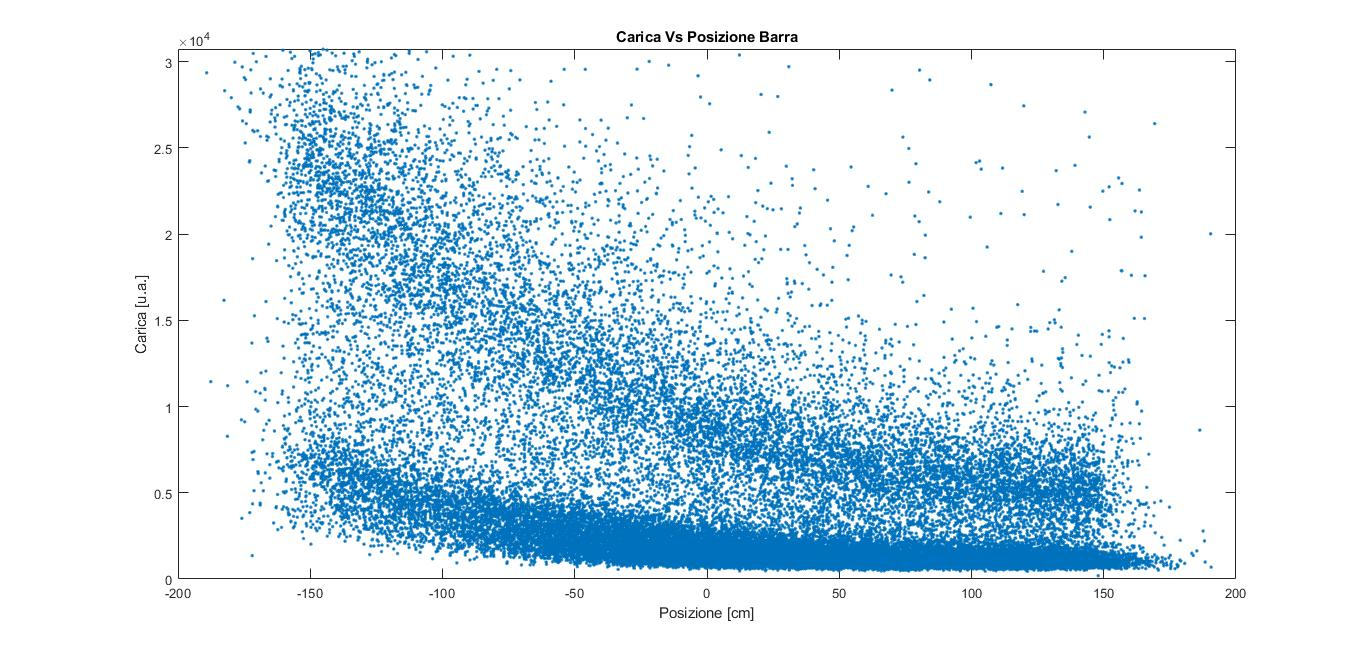
\includegraphics[width=\textwidth]{./immagini/TimeOfFlight/AttenuazioneDoppia.jpg}
\caption{}
\label{fig:AttenuazioneDoppia}
\end{subfigure}
\begin{subfigure}[b]{0.45\textwidth}
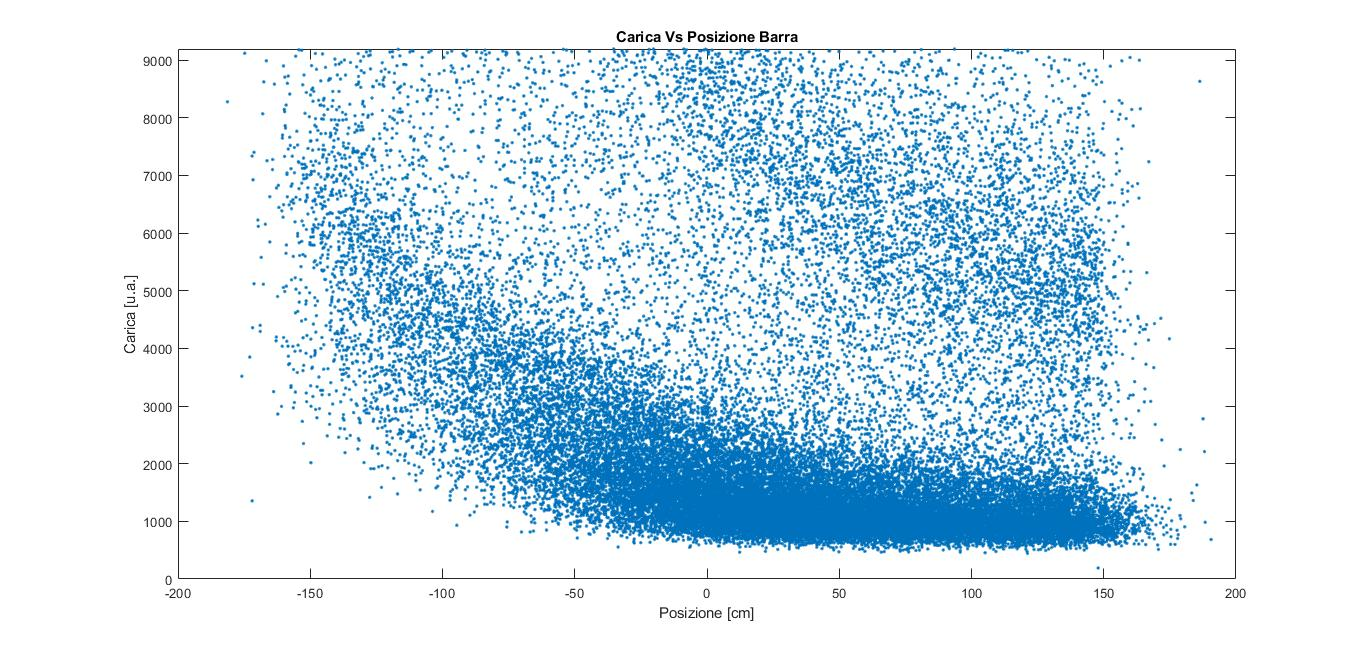
\includegraphics[width=\textwidth]{./immagini/TimeOfFlight/AttenuazioneDoppiaZoom.jpg}
\caption{Zoom sui dati inferiori}
\label{fig:AttenuazioneDoppiaZoom}
\end{subfigure}
\end{figure}

Dalla figura \ref{fig:AttenuazioneDoppia} si nota un andamento di tipo esponenziale e due zone differenti che seguono lo stesso andamento come si vede dalla figura \ref{fig:AttenuazioneDoppiaZoom}. Tutti quei segnali sappiamo non essere dipendenti dalla luce perché i conteggi in singola con luce a accesa o spenta non sono variati.\\
\'E stata fatta una prova per vedere quali fossero segnali di rumore unicamente entranti nella barra scintillante provando le coincidenze triple con gli stessi dati.

\begin{figure}[H]
\begin{subfigure}[b]{0.45\textwidth}
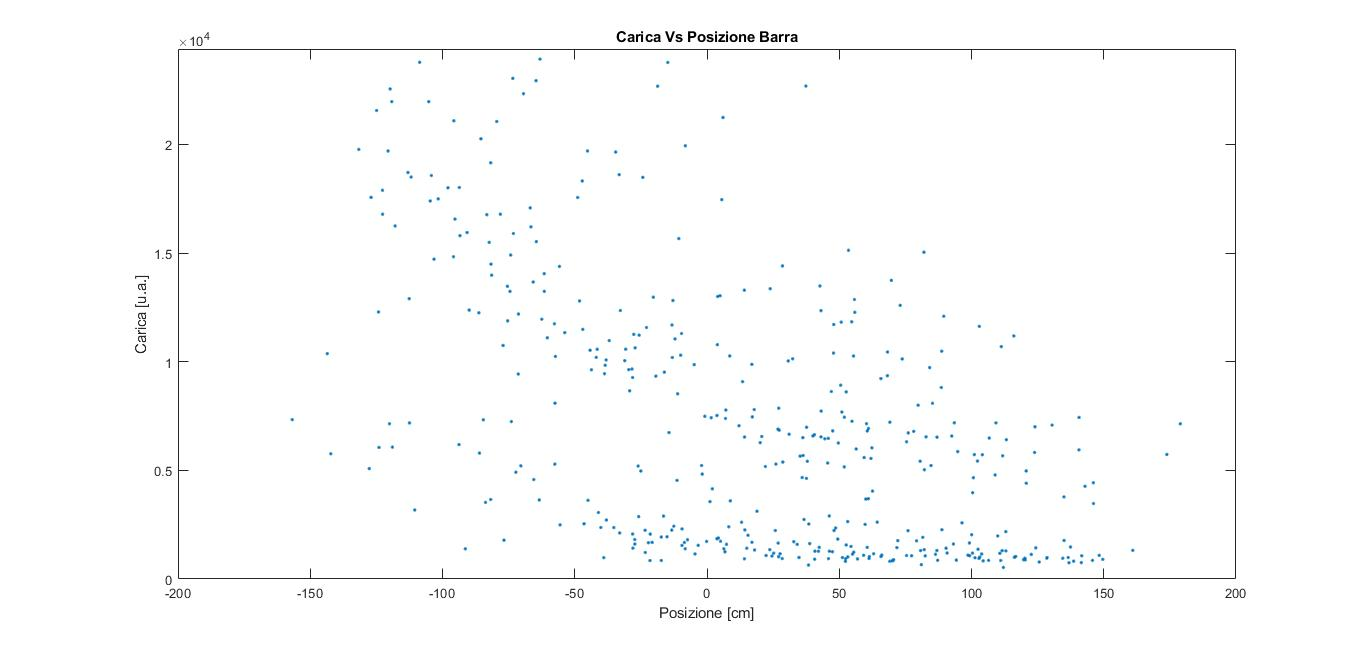
\includegraphics[width=\textwidth]{./immagini/TimeOfFlight/AttenuazioneTripla.jpg}
\caption{Coincidenze triple ricavate dai dati della figura \ref{fig:AttenuazioneDoppia}}
\label{fig:AttenuazioneTripla}
\end{subfigure}
\begin{subfigure}[b]{0.45\textwidth}
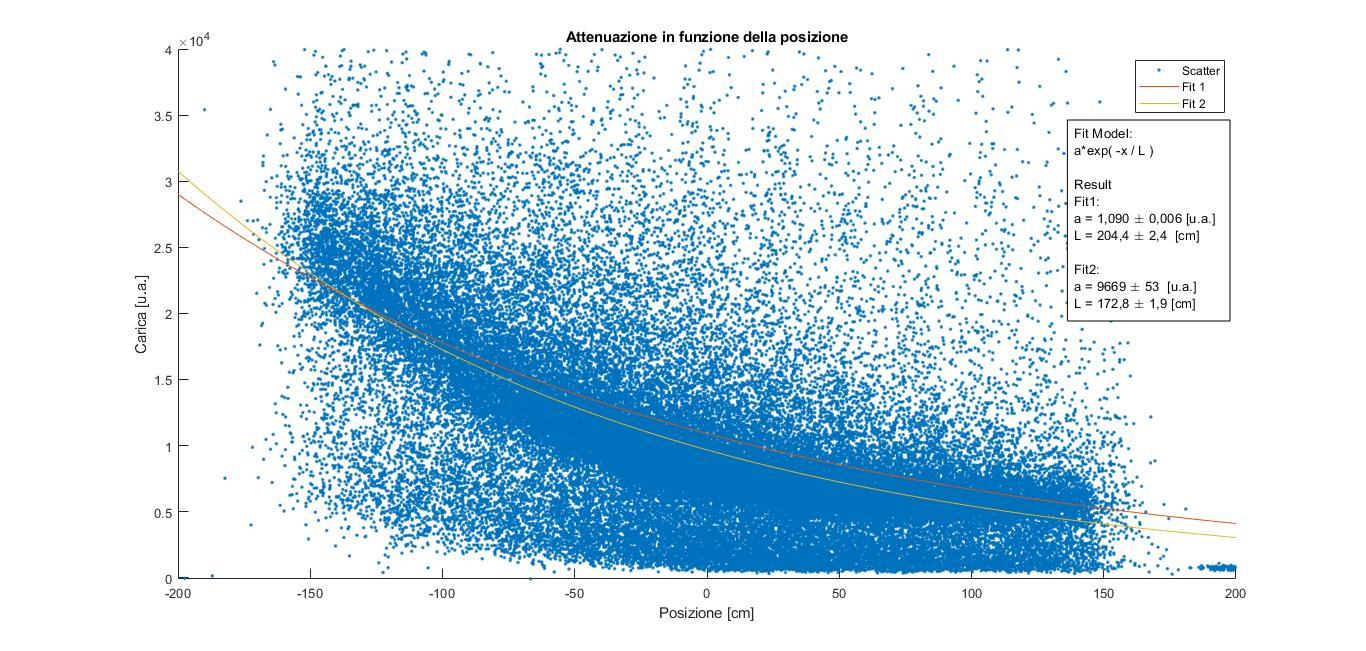
\includegraphics[width=\textwidth]{./immagini/TimeOfFlight/AttenuazioneMatlab.jpg}
\caption{Dati riferiti alle triple prese per la distribuzione di V con il piombo}
\label{fig:AttenuazioneTriplaFitta}
\end{subfigure}
\end{figure}

Nonostante il riconoscimento delle triple nei dati in figura \ref{fig:AttenuazioneDoppia} notiamo dallo scaterplot \ref{fig:AttenuazioneTripla} la presenza di segnali rivelati ad energie inferiori, e come si vede dalla figura \ref{fig:AttenuazioneTriplaFitta} questi dati sono effettivamente delle particelle passanti per il sistema poiché ottenuti tramite coincidenze triple tra i PMT(1-2-3).\\
Per valutarne effettivo andamento sono stati provati due fit con il modello di equazione \ref{eq:AttLuce}($L_0 = a$).\\
Nel caso del Fit-1 sono stati tagliati i dati a bassa intensità, nel secondo, Fit-2 sono stati considerati anche quelli.\footnote{La figura è uno zoom di tutti i dati per evidenziare la zona comprendente la quantità maggiore di dati. Ci sono alcuni dati evidentemente molto lontani dalla realtà che sono stati eliminati da entrambi i fit.}\\
I risultati segnati in figura sembrano avvicinarsi alla lunghezza di attenuazione segnata nel datasheet della barra di 210 cm

\subsection{Dipendenza dall'angolo}
Per valutare l'attenuazione del segnale luminoso all'interno della barra scintillante si deve tenere di conto anche della dipendenza dall'angolo con il quale la particella incide sulla barra\\
Per visualizzare quale fosse la dipendenza dall'angolo di incidenza della particella sulla barra è stato necessario eliminare prima la dipendenza dalla posizione. Un diverso angolo di incidenza nella barra implica un percorso della particella più o meno lungo e quindi un fascio luminoso più o meno energetico\\
Sapendo che la carica vista dal PMT-1 segue la legge:
\begin{equation}
C_1(x) = C_1 f(\theta)e^{(-\frac{\frac{L}{2}+x}{l})}
\end{equation}
mentre per il PMT-2:
\begin{equation}
C_2(x) = C_2f(\theta)e^{(-\frac{\frac{L}{2}-x}{l})}
\end{equation}
dove $f(\theta)$ è una dipendenza dall'angolo in questione. Facendo il prodotto tra le due cariche si ricava:
\begin{equation}
C_1(x)C_2(x) = f(\theta)^2 C_1C_2 e^{-\frac{L}{l}}
\end{equation}

Dove però anche $C_1$ e $C_2$ dipendono da $\theta$ e quindi il prodotto tra gli integrali del segnale diventa una funzione solo di theta.\\
Per trasformare la variabile posizione (x) in $\theta$:
\begin{equation}
\theta = arctg(\frac{h}{x})
\label{eq:XtoTheta}
\end{equation}
dove h è l'altezza della barra scintillante dal PMT-3

\begin{figure}[H]
\centering
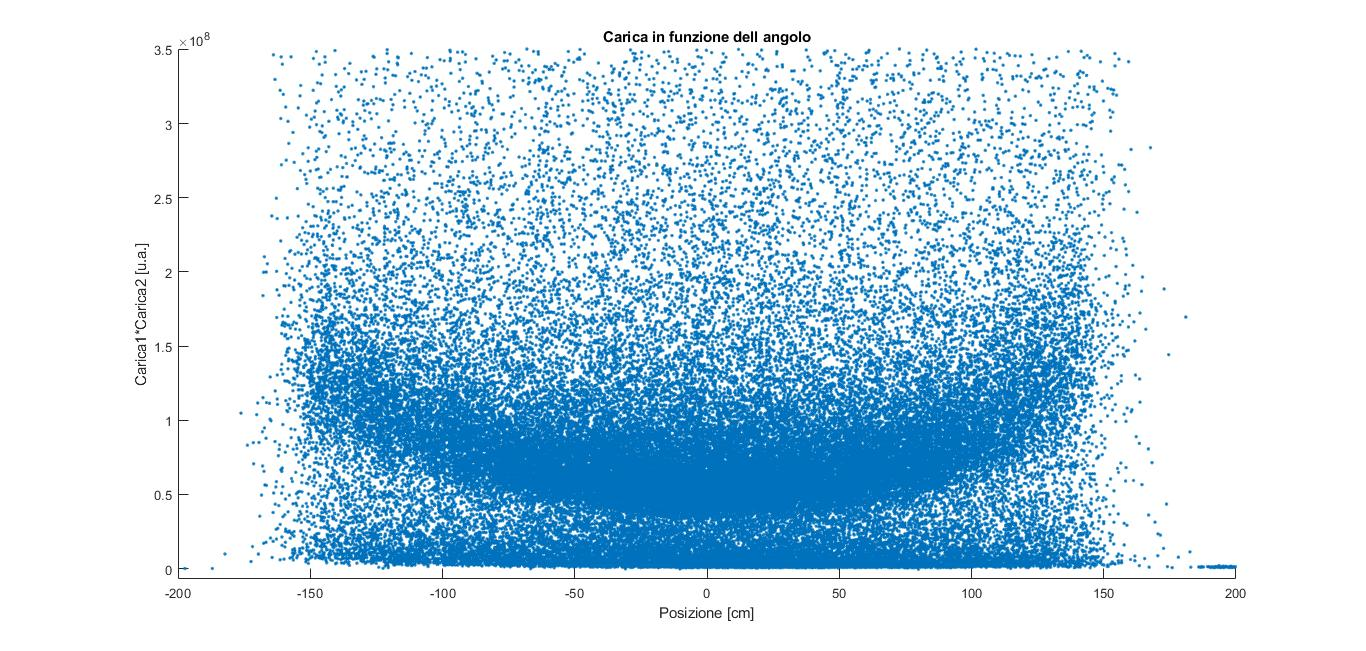
\includegraphics[scale=0.3]{./immagini/TimeOfFlight/DipendenzaAngolo.jpg}
\caption{Qua è riportata la dipendenza ancora da x ma è sufficiente un cambio di variabile \ref{eq:XtoTheta} per vedere la dipendenza dall'angolo}
\label{fig:DipendenzaAngolo}
\end{figure}

Dai dati usati in figura \ref{fig:DipendenzaAngolo} è stato inoltre possibile valutare quanti fossero gli eventi a cariche maggiori rispetto a quelli minori tramite la visualizzazione con un istogramma.\\
\'E stata stimata una percentuale di circa l' 80$\%$ di particelle con cariche maggiori rispetto al totale osservando un istogramma con il prodotto delle cariche osservate
\begin{equation}
OltreUnaSoglia [\%] = \frac{Cariche Alte}{Tot Eventi} \simeq \frac{61810}{76452} = 80 \% 
\end{equation}

\section{Altre distribuzioni}
\begin{figure}[H]
\begin{subfigure}[b]{0.4\textwidth}
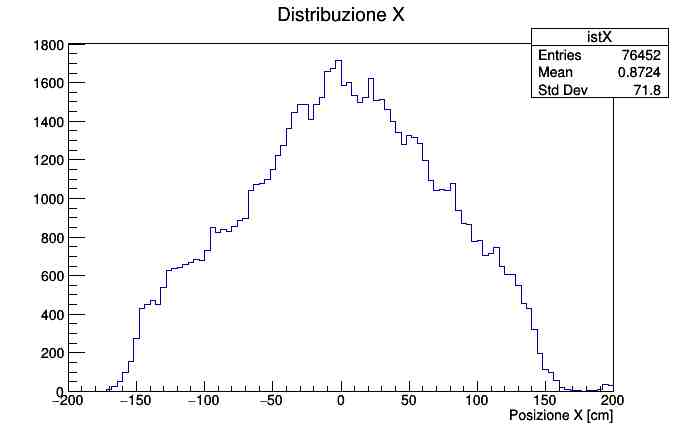
\includegraphics[width=\textwidth]{./immagini/TimeOfFlight/DistrX.jpg}
\caption{Ricavata con l'equazione \ref{eq:PosX}}
\label{fig:DistrX}
\end{subfigure}
\hfill
\begin{subfigure}[b]{0.4\textwidth}
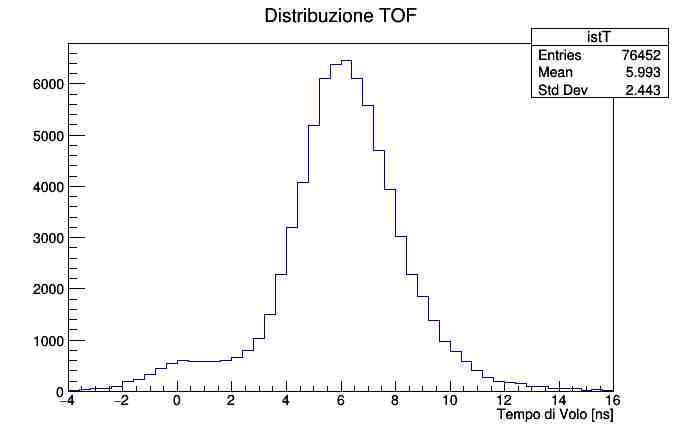
\includegraphics[width=\textwidth]{./immagini/TimeOfFlight/DistrTOF.jpg}
\caption{Tempo di volo misurato con l media tra TOF$_1$ e TOF$_2$ come in equazione \ref{eq:TOF}}
\label{fig:DistrTof}
\end{subfigure}
\end{figure}

\begin{figure}[H]
\begin{subfigure}[b]{0.4\textwidth}
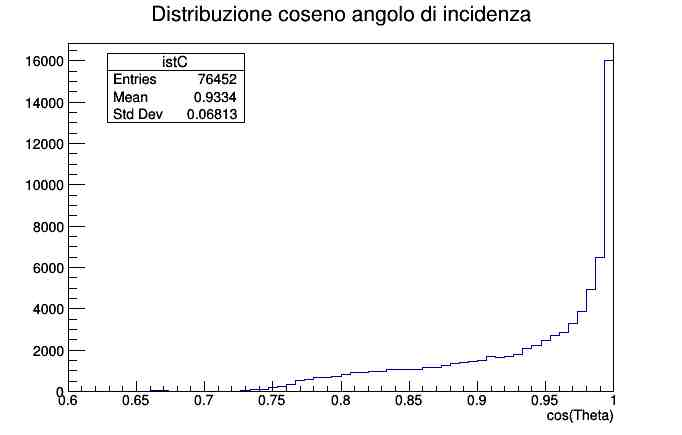
\includegraphics[width=\textwidth]{./immagini/TimeOfFlight/DistrCos.jpg}
\caption{$Cos(\theta) = \frac{x}{d}$}
\label{fig:DistrCos}
\end{subfigure}
\hfill
\begin{subfigure}[b]{0.4\textwidth}
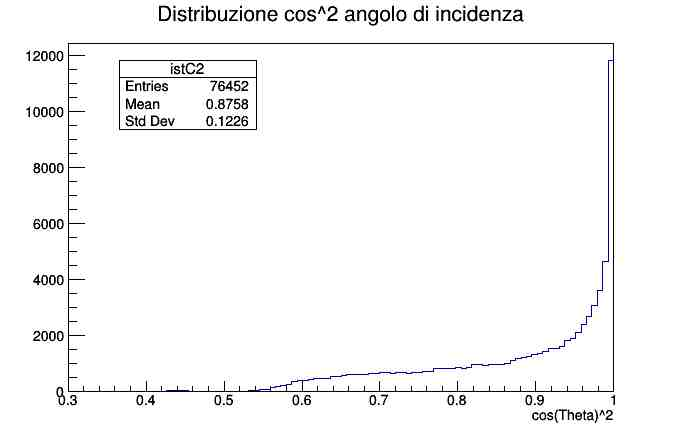
\includegraphics[width=\textwidth]{./immagini/TimeOfFlight/DistrCos2.jpg}
\caption{}
\label{fig:DistrCos2}
\end{subfigure}
\end{figure}

\section{Conclusioni}
\subsection{Proprietà barra scintillante}
\subsubsection{Velocità dei segnali}
La velocità è risultata inferiore a quella attesa ($\sim 19\frac{cm}{ns}$) probabilmente perché il fascio di luce non compie delle traiettorie lineari dal punto in cui parte fino al fotocatodo ma riflettendosi lungo le pareti della barra scintillante compie un tragitto più lungo.

\subsubsection{Attenuazione dei segnali}
Per quanto riguarda i comportamenti dell'attenuazione del segnale luminoso denella barra scintillante i due fit provati in figura \ref{fig:AttenuazioneTriplaFitta} mostrano come l'andamento possa essere buono in quanto, seppur le misure non siano accurate non sono
stati riscontrati comportamenti stravaganti.\\
Per quanto riguarda la fascia di dati a cariche inferiori, visibile in tutti i grafici di sezione \ref{sec:Atte}, sappiamo non essere solo rumore in quanto presenti anche negli scatter plot ottenuti con eventi di triple tra PMT(1-2-3) con PMT come in figura \ref{fig:PMT3posPMT4}, e sappiamo non dipendere nemmeno dalla luce poiché una semplice verifica di conteggi a luce accesa e spenta mostra una differenza veramente irrisoria.


\subsection{Distribuzione di V}
La distribuzione di V di figura \ref{fig:VFore} sembra ben centrata su una media di circa 30$\frac{cm}{ns}$ con una larghezza che non spaventa. Infatti se pensiamo che i tempi di volo per particelle relativistiche sono di circa 6-8 ns(Valori stimati e anche visibili in figura \ref{fig:DistrTof}), con errori di circa 2ns dovuti alla larghezza degli istogrammi dei ritardi(vedi per esempio \ref{tab:RitFore}) si hanno errori del 30-40$\%$, riportati sulla velocità ricaviamo un'ampiezza a metà altezza di una decina di ns. Per quanto riguarda la coda della distribuzione di V che troviamo per velocità molto maggiori della luce non sembra implicata ad un'incorretta stima della posizione di incidenza ma piuttosto ad errori nella distribuzione di TOF (Vedi \ref{fig:DistrX} per la posizione e \ref{fig:DistrTof} per il tempo di volo).\\
La normalizzazione sembra essere corretta ed equa in entrambi i casi con e senza Piombo in quanto gli integrali della distribuzione valgono entrambi 0,97
\subsubsection{Particelle Relativistiche e non}
\paragraph{Metodo 1}
Dai risultati ottenuti con il primo metodo si nota dalla figura \ref{fig:VRappFore} che le particelle con velocità inferiori a 10$\frac{cm}{ns}$ sembrano essersi fermate nel piombo non raggiungendo il PMT-4, questo potrebbe aver determinato l'aumento della velocità media da 29,6$\pm$6,9 a 30,1$\pm$7,3 $\frac{cm}{ns}$; un aumento dell' 1,6$\%$ sulle medie stimate.\\
Quello che invece non piace sono le velocità comprese tra 10 e 20 $\frac{cm}{ns}$. In questa regione seppur gli errori sulle misure siano abbastanza grandi dovremmo aver visto una salita verso un rapporto pari ad 1 cosa che invece non si riesce a vedere

\begin{figure}
\centering
\title{Zoom della distribuzione di V}
\begin{center}
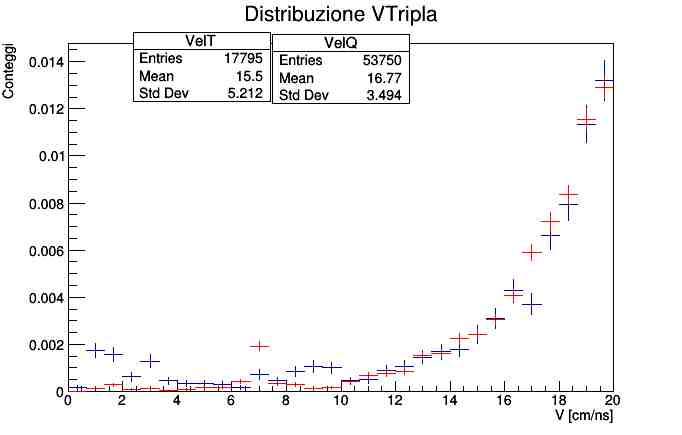
\includegraphics[scale=0.3]{./immagini/TimeOFFlight/ZoomVel.jpg}
\caption{I dati in figura corrispondono a circa il 7$\%$ di tutti i dati presi. Le prese dati sono durate da uno (per quelli Blu, senza piombo) a 3 giorni (per quelli rossi con il piombo)}
\label{fig:ZoomV}
\end{center}
\end{figure}

Facendo uno zoom sulle velocità minori di 20, vedi immagine \ref{fig:ZoomV}, si vede come data la statistica degli eventi entri in gioco in quanto troviamo in proporzione per alcune velocità (come 6 o 17$\frac{cm}{ns}$) più eventi che hanno passato il piombo di quelli che effettivamente lo potrebbero aver raggiunto dall'alto (quindi che sono arrivati al PMT3)

\paragraph{Metodo 2}
Per questo secondo metodo mettiamo a confronto le figure in sezione \ref{sec:Met2}.\\
Partiamo direttamente dal rapporto tra quadruple e triple di figura \ref{fig:RappPbFore}, come nella situazione precedente descritta nel precedente paragrafo troviamo che per v$<10\frac{cm}{ns}$ la curva tende con alta incertezza a restare più bassa di 1. la maggior differenza si nota per velocità maggiori di 40$\frac{cm}{ns}$ dove si nota come il rapporto scende gradualmente sotto l'unità del rapporto $\frac{quadruple}{triple}$.\\
Se confrontiamo questi effetti con il grafico per l'efficienza del PMT-4, figura \ref{fig:EffPMT4}, si nota che per velocità basse si ha molta confusine enon si può definire un andamento o un comportamento particolare, mentre per alte velocità si ha nuovamente una discesa. Infatti osservando il rapporto $\frac{quadruple}{triple}$ corretto con l'efficienza, figura\ref{fig:RappPbEffFore}, si può dire come l'efficienza abbia corretto ed influenzato maggiormente la regione di velocità ultrarelativistiche mentre lascia invariata la zona a v<10$\frac{cm}{ns}$.\\
Infine osservando le distribuzioni di velocità in figura \ref{fig:DistrVPb2Fore} si nota una differenza tra gli integrali misurati sotto la curva: 0,93 per la distribuzione di v delle triple, mentre 0,98 per la distribuzione di v delle quadruple.\\
Quello che si ptrebbe andare ad affermare è che il Piombo potrebbe aver frenato alcune particelle a bassa velocità, in particolare però al di sotto dei 10$\frac{cm}{ns}$ piuttosto che di 20$\frac{cm}{ns}$, mentre l'efficienza del PMT-4 abbia influenzato le particelle ultrarelativistiche facendo inoltre incrementare il peso del numero di particelle nelle distribuzioni normalizzate, ciò ha fatto si che, nella validità dell'analisi effettuata, si ottenesse un numero maggiore di quadruple che di triple e l'effetto dell'efficienza non abbia influenzato il comportamento dei dati per basse velocità









\newpage
\appendix
\section{Problemi affrontati}
\label{secA:ProblemiADC}
La procedura seguita per migliorare i nostri calcoli e individuare gli errori parte dal riconoscimento dell'evento presumibilmente ricostruito male o che riporta come risultato una velocità molto lontana dalle aspettative. Dopo l'individuazione di uno di questi eventi semplicemente si visualizza con un semplice plot dei dati dell'evento e interpretandolo si prova a capire quale possa essere il problema in analisi o in presa dati che ha portato a quell'errore.\\
Alcuni errori sono stati commessi nei codici di analisi dati e successivamente rimossi, altri invece sono stati causati dalle caratteristiche dell'ADC.\\
Qua sono riportate alcune correzioni e errori commessi in ordine di come sono stati trovati.\\
Durante la descrizione dei problemi saranno indicate alcune delle funzioni scritte e utilizzate per l'analisi dati, spero di inserire il link del repositorio online per una visualizzazione

\subsection{Lunghezza record Dati "ADC Record Lenght"}
\label{secA:RecLenght}
Il primo problema è legato alla lunghezza del record di dati che l'ADC restituisce ogni qual volta scatti il trigger impostato generalmente su una tripla C$_{123}$.\\
Una delle cause che faceva risultare una particella ultrarelativistica era che nello stesso record di dati non vi era solo l'evento triggerante ma anche un secondo evento (a volte una doppia o anche un segnale rivelato in un unico PMT). Questa "coincidenza casuale" faceva si che il codice di analisi dati riportasse come $\Delta t$ un intervallo di tempo tra due impulsi relativi a due eventi diversi e non allo stesso.\\
Infatti facendo un semplice conto la possibilità che due eventi fossero registrati nello stesso record di dati non è così bassa.\\
Partiamo dal fatto che un record è lungo 1030 punti, cioè, sapendo che l'ADC campiona con una frequenza di 250MHz ogni campione disterà temporalmente dai vicini 4 ns, e quindi in totale si ha una finestra in tempi di 4,12 $\mu$s. Andando a calcolare le coincidenze casuali con questa finestra temporale di 4$\mu$s si ottiene:

\begin{equation}
f_{cas} = f_1*f_1*\tau = 10^4*10^{-6} = 10^{-2}
\end{equation}

cioè 1 ogni 100 eventi potrebbe presentare due eventi su un unico record di dati che dovrbbe corrispondere ad una sola tripla, ad un solo evento.\footnote{In questo calcolo teniamo di conto di un solo Scintillatore e dell'ordine di grandezza dei cps di quest'ultimo, e nel caso in questione, per le scelte fatte per eseguire il conto, le coincidenze possono solo aumentare.}
Per rimediare a questo problema è stato pensato di scrivere una funzione che funzionasse come un trigger sui dati da analizzare, questo ha permesso di trovare eventuali coincidenze tra segnali provenienti da PMT che non erano messi in coincidenza tramite il modulo NIM apposito.\\
Per riuscire in questo è stato necessario discriminare i minimi relativi dei record di dati e discriminare i minimi di rumore da quelli dovuti a particelle.\\
Facendo questa operazione è stato possibile eliminare segnali come quelli in figura \ref{fig:FalsaTripla}

\begin{figure}[H]
\centering
\title{Falsa tripla}
\begin{center}
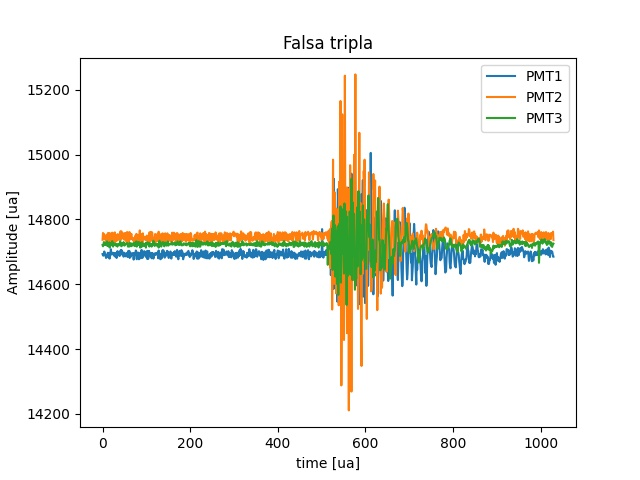
\includegraphics[scale=0.4]{./immagini/TimeOfFlight/FalsaTripla.jpg}
\caption{Sono stati trovati con percentuali sotto l'1$\%$ segnali di questo tipo in tutte le prese dati}
\label{fig:FalsaTripla}
\end{center}
\end{figure}

\subsection{Ricerca dei minimi, Threshold}
\label{secA:Threshold}
Più volte in analisi dati come visto precedentemente (\ref{secA:RecLenght}) è stato necessario determinare una certa soglia per discriminare quale fosse un minimo del segnale, oppure quale fosse l'inizio o la fine di un segnale.
\paragraph{Function: GestioneOff}
Ogni evento ricostruito dall'ADC si presentava rialzato dallo 0 di un offset di circa 14700 ua. Per sistemare questo offset è stato necessario settare delle soglie molto intuitive per decidere quali dati fossero di rumore e quali di un segnale.\footnote{In realtà ne sono state settate 2 una superiore e una inferiore, il perché sarà spiegato più avanti} Da questa prima discriminazione è stato ricavato un offset(media dei valori del rumore) e una sigma (deviazione standard di questi valori). Questa sigma è stata usata per discriminare i dati di un segnale da quelli di rumore.
\paragraph{Function: ThrsDet}
Un'altra idea per ricercare i minimi relativi dei record\footnote{Per la ricerca dei minimi relativi sono state provate due funzioni ugualmente funzionanti, una scritta individualmente e un'altra che è la funzione find$\_$peaks contenuta nel modulo python scipy.signal} è stata quella di valutare quante sigma entrassero dentro il minimo assoluto di ogni record di dati cioè fare il rapporto:

\begin{center}
$\frac{Sigma}{Absolute min}$
\end{center}

è stato scelto di fare un istogramma di questi risultati e selezionare una soglia il più bassa possibile per perdere meno eventi possibile\footnote{Come si vede nelle funzioni ...Recognize() è stata scelta per tutti i PMT una soglia di 15 Sigma}.


\subsection{Miglioramenti e tentativi}
\label{sec:Tentativi}
L'altra limitazione che è stata affrontata è quella dovuta al rate di campionamento dell'ADC.\\
L'ADC N6725S campiona con una frequenza di 250MHz cioè un campione ogni 4 ns e sapendo che i segnali sono in media lunghi dai 15 a 20 ns e sono di tipo impulsivo, la ricostruzione di questi, in particolare del picco, da parte dello strumento non è ottimale.

\paragraph{Time stamp}
Di solito con time-stamp di un segnale impulsivo si considera l'istante in cui esso raggiunge il 50$\%$ in ampiezza del valore minimo del segnale. Inoltre si considera inizio e fine del segnale quando questi sono compresi rispettivamente tra il 10$\%$ e il 90$\%$.\\
Queste due operazioni però non sono state possibili in quanto determinati segnali impulsivi raggiungevano il minimo partendo da sotto il 10$\%$ con un solo dato dell'ADC, cioè con un tempo inferiore a 4ns e questo valeva sia per segnali poco energetici che per alcuni molto energetici che non venivano riconosciuti dalle funzioni.\\
Per misurare il TimeStamp sono state fatte diverse prove, se ne mostrano le differenze tramite gli istogrammi dei ritardi tra le trasmissioni di PMT-2 e PMT-1 e la distribuzione di V\footnote{il calcolo di TimeStamp ha una propria funzione TimeStampMeas. Inoltre le funzioni che determinano l'inizio e la fine di un segnale che utilizzano la sigma si chiamano findstart e findstop}

\begin{figure}[H]
     \centering
     \title{Media della discesa del segnale}
     \begin{center}
     \begin{subfigure}[b]{0.4\textwidth}
         \centering
         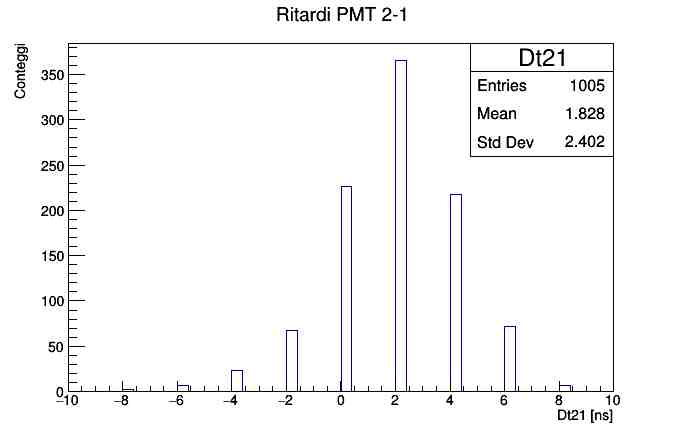
\includegraphics[width=\textwidth]{./immagini/TimeOfFlight/Rit21MidNegSlo.jpg}
         \caption{}
         \label{fig:Dt21MidNegSlo}
     \end{subfigure}
     \hfill
     \begin{subfigure}[b]{0.4\textwidth}
         \centering
         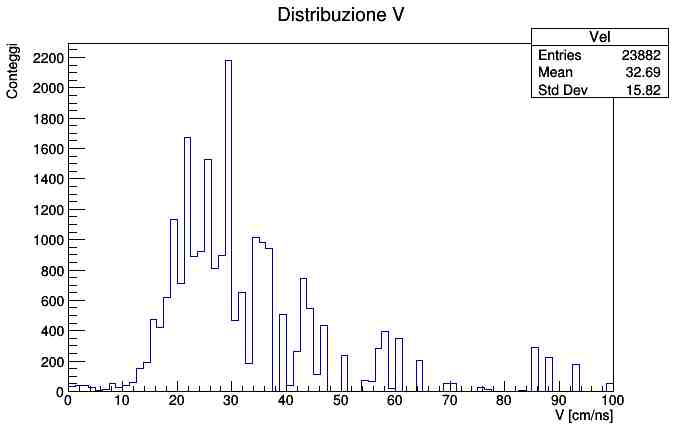
\includegraphics[width=\textwidth]{./immagini/TimeOfFlight/VMidNegSlo.jpg}
         \caption{}
         \label{fig:VMidNegSlo}
     \end{subfigure}
     \end{center}
     \caption{Per fare queste misure i time stamp sono stati valutati prendendo il punto medio del tempo di discesa del segnale senza eliminare i punti sopra il 90$\%$ e sotto il 10$\%$. Quindi a partire dal primo punto distante più di una sigma fino al minimo}        
     \label{fig:MidNegSlo}
\end{figure}

\begin{tabular}{c|c|c}
Rit 2-1 [ns] & Rit 3-1 [ns] & Rit 3-2 [ns] \\
\hfill
2,13 $\pm$ 2,25 & -9.07 $\pm$ 2,19 & -11,0 $\pm$ 2,53
\hfill
\label{tab:RitMidNegSlo}
\end{tabular}

I dati sono eccessivamente discreti e la riproduzione di V troppo larga e con picchi troppo marcati

\begin{figure}[H]
     \centering
     \title{Baricentro della discesa del segnale}
     \begin{center}
     \begin{subfigure}[b]{0.4\textwidth}
         \centering
         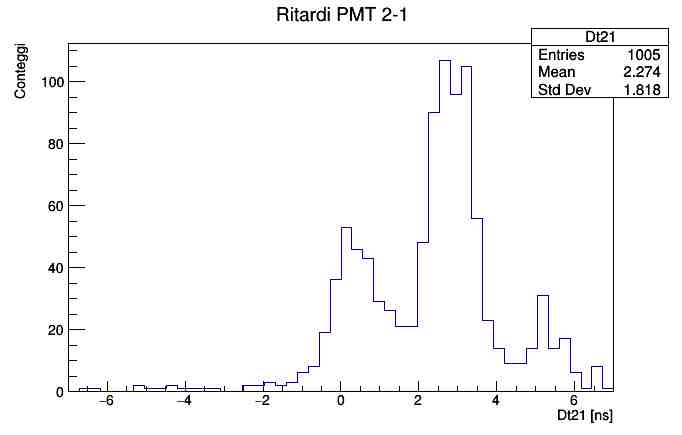
\includegraphics[width=\textwidth]{./immagini/TimeOfFlight/Rit21IntNegSlo.jpg}
         \caption{}
         \label{fig:Dt21IntNegSlo}
     \end{subfigure}
     \hfill
     \begin{subfigure}[b]{0.4\textwidth}
         \centering
         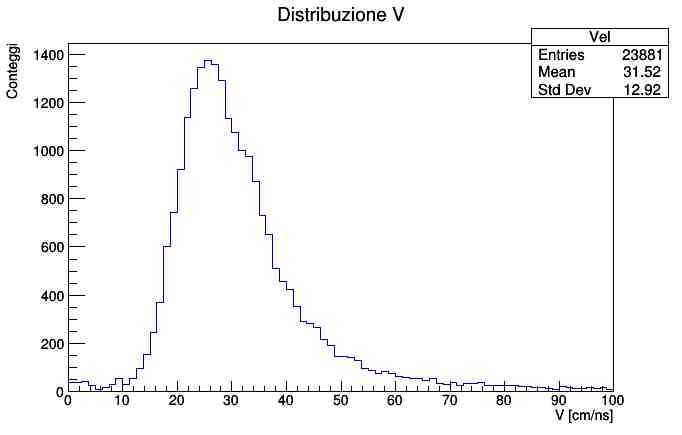
\includegraphics[width=\textwidth]{./immagini/TimeOfFlight/VIntNegSlo.jpg}
         \caption{}
         \label{fig:VIntNegSlo}
     \end{subfigure}
     \end{center}
     \caption{Per fare queste misure i time stamp sono stati valutati prendendo il baricentro della parte di segnale dalla partenza fino al minimo}        
     \label{fig:IntNegSlo}
\end{figure}

\begin{tabular}{c|c|c}
Rit 2-1 [ns] & Rit 3-1 [ns] & Rit 3-2 [ns] \\
\hfill
2,23 $\pm$ 1,72 & -9.47 $\pm$ 1.81 & -11,7 $\pm$ 2,06
\hfill
\label{tab:RitIntNegSlo}
\end{tabular}

\begin{figure}[H]
     \centering
     \title{Baricentro del segnale}
     \begin{center}
     \begin{subfigure}[b]{0.4\textwidth}
         \centering
         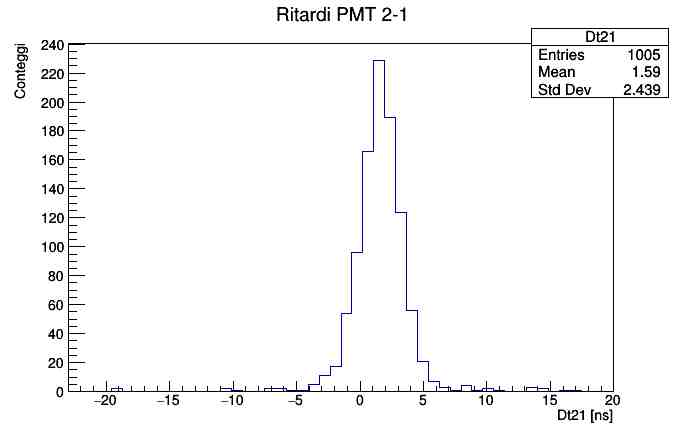
\includegraphics[width=\textwidth]{./immagini/TimeOfFlight/Rit21IntSinTot.jpg}
         \caption{}
         \label{fig:Dt21IntSigTot}
     \end{subfigure}
     \hfill
     \begin{subfigure}[b]{0.4\textwidth}
         \centering
         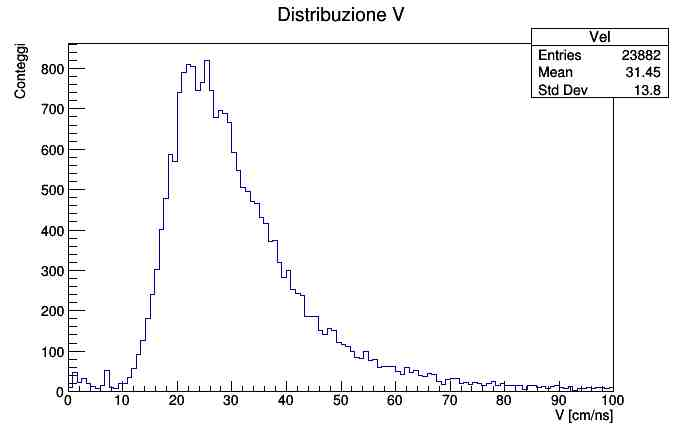
\includegraphics[width=\textwidth]{./immagini/TimeOfFlight/VIntSigTot.jpg}
         \caption{}
         \label{fig:VIntSinTot}
     \end{subfigure}
     \end{center}
     \caption{Per fare queste misure i time stamp sono stati valutati prendendo il baricentro di tutto il segnale ovvero dal primo valore oltre una sigma dallo zero e fino all'ultimo trovato}        
     \label{fig:IntSinTot}
\end{figure}

\begin{tabular}{c|c|c}
Rit 2-1 [ns] & Rit 3-1 [ns] & Rit 3-2 [ns] \\
\hfill
1,58 $\pm$ 1,56 & -13,3 $\pm$ 2,07 & -14,9 $\pm$ 2,13
\hfill
\label{tab:RitIntSigTot}
\end{tabular}

L'intento è quello di ricercare il momento in cui passa il segnale per intero

\begin{figure}[H]
     \centering
     \title{Baricentro del segnale con qualche dato in più}
     \begin{center}
     \begin{subfigure}[b]{0.4\textwidth}
         \centering
         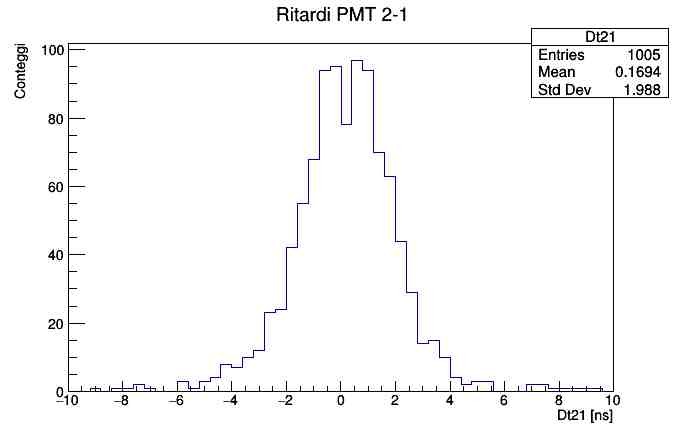
\includegraphics[width=\textwidth]{./immagini/TimeOfFlight/Rit21Largo.jpg}
         \caption{}
         \label{fig:Dt21Largo}
     \end{subfigure}
     \hfill
     \begin{subfigure}[b]{0.4\textwidth}
         \centering
         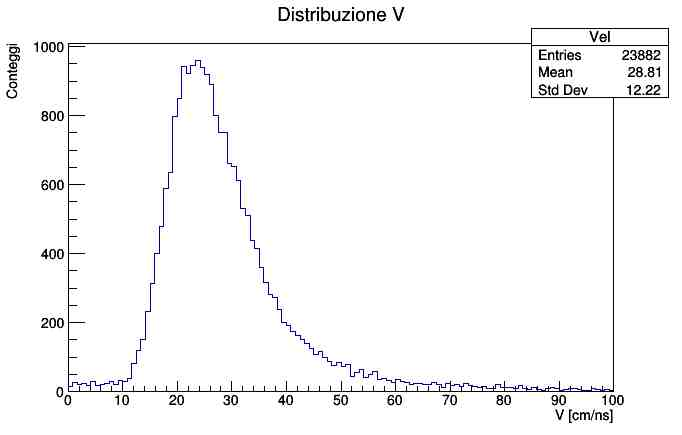
\includegraphics[width=\textwidth]{./immagini/TimeOfFlight/VLargo.jpg}
         \caption{}
         \label{fig:VLargo}
     \end{subfigure}
     \end{center}
     \caption{Per fare queste misure i time stamp sono stati valutati prendendo il baricentro di tutto il segnale considerando l'inizio e la fine 5 unità di tempo in più, cioè 20 ns sia a destra che a sinistra del segnale}        
     \label{fig:Largo}
\end{figure}

\begin{tabular}{c|c|c}
Rit 2-1 [ns] & Rit 3-1 [ns] & Rit 3-2 [ns] \\
\hfill
0,19 $\pm$ 1,64 & -14,8 $\pm$ 2,17 & -14,9 $\pm$ 2,31
\hfill
\label{tab:RitLargo}
\end{tabular}

Aumentando il range rispetto al caso in figura \ref{fig:IntSinTot} si vuole mediare qualche cattivo comportamento da parte del segnale

\begin{figure}[H]
     \centering
     \title{Baricentro della discesa del segnale con qualche dato in più}
     \begin{center}
     \begin{subfigure}[b]{0.4\textwidth}
         \centering
         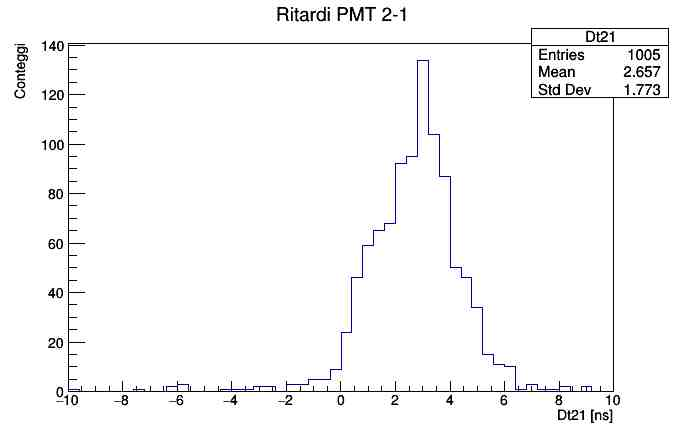
\includegraphics[width=\textwidth]{./immagini/TimeOfFlight/Rit21Fore.jpg}
         \caption{}
         \label{fig:Dt21ForeA}
     \end{subfigure}
     \hfill
     \begin{subfigure}[b]{0.4\textwidth}
         \centering
         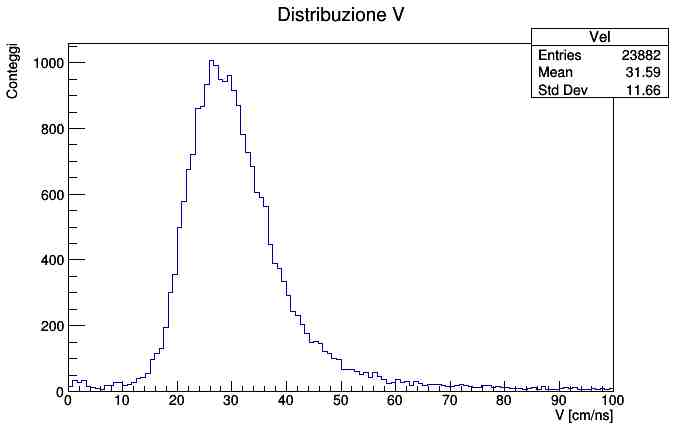
\includegraphics[width=\textwidth]{./immagini/TimeOfFlight/VFore.jpg}
         \caption{}
         \label{fig:VForeA}
     \end{subfigure}
     \end{center}
     \caption{Per fare queste misure i time stamp sono stati valutati prendendo il baricentro della discesa negativa del segnale considerando quindi come inizio l'inizio del segnale più un'unità di tempo, mentre come fine il minimo del segnale più 3 punti}        
     \label{fig:ForeA}
\end{figure}

\'E stata fatta questa prova per rimanere il più fedeli possibile alla definizione di TimeStamp e considerare una parte di segnale equa per tutti i segnali, nonostante questi non abbiano alcune volte un picco ben riprodotto, inoltre in questa maniera non si considerano nel conto dell'integrale alcuni ringing del segnale successivi al minimo di esso 

\begin{tabular}{c|c|c}
Rit 2-1 [ns] & Rit 3-1 [ns] & Rit 3-2 [ns] \\
\hfill
2,74 $\pm$ 1,42 & -10,0 $\pm$ 1,48 & -12,8 $\pm$ 1.65
\hfill
\label{tab:RitForeA}
\end{tabular}



\subsection{Scelta}
\label{secA:Scelta}
La scelta tra i vari metodi di calcolo del TimeStamp è stata fatta considerando i risultati ottenuti tramite fit delle distribuzioni dei ritardi tra i PMT e la relativa ricostruzione della distribuzione di V.\\
\'E stato scelto di utilizzare il metodo tramite integrazione di una parte più ampia della discesa del segnale, in particolare 4ns(1 campione dell'adc) prima dell'inizio del segnale e 12 ns dopo il minimo di esso (3 campioni otre).\\
In questa maniera oltre che rimanere fedeli alla definizione di TimeStamp si considera una parte di segnale che a meno di ampiezza differenti che, nel caso della ricerca del baricentro non influisce in modo determinante, rimane molto simile tra i vari segnali. Inoltre si potrebbero mediare eventuali problemi di ricostruzione del picco e alcuni fastidiosi ringing che può presentare il segnale

\section{Repositorio}
Ho inserito un repositorio online al link:\\
\url{https://github.com/AndreaForesi/Laboratorio-Interazioni-Fonddamentali-20-21}\\
Verificarne l'aggiornamento e la riutilizzabilità

\end{document}